\documentclass[useAMS,usenatbib,twocolumn]{mn2e}

%\addtolength{\marginparwidth}{1.875in}

\usepackage{graphicx}
\usepackage{dcolumn}
\usepackage{bm}
\usepackage{listings}
\usepackage{amssymb}
\usepackage{verbatim}
\usepackage{url}
% \usepackage{amsthm}
\usepackage{mathtools}
\usepackage{amsmath}
\usepackage{longtable}
\usepackage{booktabs}
\usepackage{ctable}
% \usepackage{natbib}
% \bibliographystyle{apj}

% Symbol
\makeatletter
\newcommand{\HI}{{\rm H\,{\scriptstyle I}}}
\newcommand{\HII}{{\rm H\,{\scriptstyle II}}}
\newcommand{\HeI}{{\rm He\,{\scriptstyle I}}}
\newcommand{\HeII}{{\rm He\,{\scriptstyle II}}}
\newcommand{\HeIII}{{\rm He\,{\scriptstyle III}}}
\newcommand{\rmnum}[1]{\romannumeral #1}
\newcommand{\Rmnum}[1]{\expandafter\@slowromancap\romannumeral #1@}
\newcommand{\nHI}{n_{\mbox{\tiny H\Rmnum{1}}}}
\newcommand{\xHI}{x_{\mbox{\tiny H\Rmnum{1}}}}
\newcommand{\xHII}{x_{\mbox{\tiny H\Rmnum{2}}}}
\newcommand{\eHI}{\epsilon_{\mbox{\tiny H\Rmnum{1}}}}
\newcommand{\LyA}{\mbox{Ly}\alpha}
\newcommand{\fHI}{\langle f_{\mbox{\tiny H\Rmnum{1}}}\rangle}
\newcommand{\fHII}{\langle f_{\mbox{\tiny H\Rmnum{2}}}\rangle}
\newcommand{\NHI}{N_{\mbox{\tiny H\Rmnum{1}}}}
\newcommand{\NHIi}{N_{\mbox{\tiny H\Rmnum{1}},i}}
\makeatother

%Journals
\newcommand{\aap}{A\&Ap}
\newcommand{\aj}{AJ}
\newcommand{\apj}{ApJ}
\newcommand{\apjl}{ApJ}
\newcommand{\apjs}{ApJS}
\newcommand{\araa}{ARA\&A}
\newcommand{\mnras}{MNRAS}
\newcommand{\physrep}{Phys. Rep.}
\newcommand{\nat}{Nature}


\title[$\LyA$ forests and $\LyA$ galaxy surveys]
  {Joint analysis of galaxy redshift surveys and $\LyA$ forests \Rmnum{1}: \newline
  the large-scale gasenous environment of $\LyA$ galaxies 
  with redshift-space distortion}


\author[K. Kakiichi et al.]
{Koki Kakiichi et al,$^{1}$\thanks{E-mail: kakiichi@mpa-garching.mpg.de}
\\
$^1$Max Planck Institute for Astrophysics, Karl-Schwarzschild Stra\ss e 1, 85741 Garching, Germany
}


\date{Released 2002 Xxxxx XX}

\pagerange{\pageref{firstpage}--\pageref{lastpage}} \pubyear{2002}

\def\LaTeX{L\kern-.36em\raise.3ex\hbox{a}\kern-.15em
    T\kern-.1667em\lower.7ex\hbox{E}\kern-.125emX}

\begin{document}

\maketitle

\begin{abstract}
Redshift surveys of $\LyA$ forests and $\LyA$-emitting/absorbing galaxies. 
\end{abstract}

\begin{keywords}
atomic processes -- cosmology:\ theory -- line:\ formation -- radiative
transfer -- infrared:\ general -- scattering
\end{keywords}

\section{Introduction}
We propose and the explore the potentials of deep redshift surveys
of $\LyA$ galaxies in the foregound of QSOs covering redshifts $2<z<7$.
Joint analysis of $\LyA$ forests and $\LyA$-emitting and absorbing galaxies
over redshift $2<z<7$ enables us to investigate the Epoch of Reionization
and the transition to post-reionization era, allowing to break the multiple 
degeneracies arising from analysis of high-redshift $\LyA$ galaxies alone.
For both Lyman-break and narrow-band selection technique, $\LyA$ line can 
appear in galaxies both as emission or absorption.

The gasenous environment of galaxies is a natural consequence arising from 
the concordance hierarchical structure formation in $\rm{\Lambda CDM}$
cosmology, forming cosmic web. One effect of gasenous environment on
galaxies is the impact on their formation and evolution (Dekel+),
for example, the popular cold stream picture in the formation of galaxies 
to name a few. Another important impact of the environment is to induce
the selection bias on the observation of galaxies. Since we see galaxies
through their gasenous environments, any absorption or reprocessing of the light
along a line of sight introduces the environmentally-induced selection bias 
upon observations of galaxies. One notable example of such selection bias is 
on the population of $\LyA$-emitting galaxies, which has been used to 
constrain the neutral fraction of the universe during the EoR. 
Furthermore, even at the post-reionized universe, the possibile impact 
on LAEs clustering due to the $\LyA$ RT through the gasenous environment 
as CGM and IGM (Zheng+; Wyithe \& Dijkstra; Breg+) calls for the close 
examination and testing this hypothesis based on observations. The degree of 
the environmetal impact on the LAE selection influences the interprelation of 
redshift BAO survey such as HETDEX to do cosmology (Wyithe\&Dijkstra, Breg+). 
 
The galaxy redshift survey in the foreground of QSOs is not a new
idea, which has been conducted by Aldelberger+, Cooke+, Keck Baryonic
Structure Survey (KBSS, Steidel+) for $z\sim2-3$. Yet, the connection
to EoR and RT studies of galaxies and the IGM are not or only weakly made.
The idea to perform the joint analysis of $\LyA$ galaxies and QSO spectra
occasionally has appeared in the literature (Baek, Ferrara \& Semelin 2012,
SDSS J1335+3533 good candidate?). Yet, the full potential of such survey
strategy and the requirement still must be worked out.
An idea is to extend such survey strategy to higher redshifts, which
enable us the joint analysis of LLS/DLA, $\LyA$ forests and galaxies for
both $\LyA$ in emission and absorption.



\section{Theory: Joint model of redshift space distortion and 
$\LyA$ RT}
Our primary motive is to study the intergalactic environment of $\LyA$-galaxies 
and its impact on $\LyA$ RT. The $\LyA$ RT effect on the $\LyA$-galaxy depends
on the clustering and pairwise velocity statistics between galaxies and
small-scale absorbers. We consider how to constrain the pairwise velocity
staitistics from redshift-space distortion. To build the intuition, 
we first employ the analytic theory
to connect the statistical formulations of the redshift-space 
anistoropy of galaxy-absorber systems and the cosmological $\LyA$ radiative 
transfer. The formalism for the redshift-space distortion largely follows
that by \cite{1994MNRAS.267..927F} and \cite{2011MNRAS.417.1913R}. 
The joint model will be used as an estimator to infer the pairwise velocity
distribution and it impact on the $\LyA$ visibility.

\subsection{Dynamics and statistics: galaxy-absorber pairs}
The dynamics of galaxy-absorber system and the real-space clustering form the
basis of joint statistical formulation of redshift-space anistorpy and 
$\LyA$ RT. The dynamical discription of the galaxy-absorber pairs
is provided by the phase-space information. The phase space distribution 
function of a pair is $f(v_{12},r_{12})dr_{12}dv_{12}$, i.e. the number of 
galaxy-absorber pair in the interval from $r_{12}$ to $r_{12}+dr_{12}$ 
and $v_{12}$ to $v_{12}+dv_{12}$, where $v_{12}$ is
the pairwise relative velocity between galaxy and absorber and $r_{12}$ is
the galaxy-absorber comoving distance. Because of statistical isotropy and
homogeneity, it only depends on the magnitude of pairwise velocity and
comoving seperation. 

The real-space correlation function $\bar{n}^2\xi(r)=\int f(v,r)dv$ (check).

\subsubsection{real-space clustering}
The global abundance of absorber is characterized by the column density 
distribution function $\frac{\partial\mathcal{N}}{\partial\NHI\partial z}$.
In the following treatment, it is more covenient to consider the 
CDDF per comoving distance $\left|\frac{dz}{dr}\right|
\frac{\partial^2\mathcal{N}}{\partial\NHI \partial z}$ 
where $\left|\frac{dz}{dr}\right|=c/H_0[\Omega_m(1+z)^3+\Omega_\Lambda]^{1/2}$.
Recalling the definition of correlation function, the probability find
an absorber along a one-dimensional skewer from galaxy at comoving distance 
$r$ is given by
\begin{eqnarray}
P(r)dr&=&\int d\NHI\left|\frac{dz}{dr}\right|
\frac{\partial^2\mathcal{N}}{\partial\NHI \partial z}
\left[1+\xi(r,\NHI)\right]dr, \nonumber \\
&=&\lambda_a\left[1+\bar{\xi}(r)\right]dr,
\end{eqnarray}
where the prefactor $\lambda_a(z)=\int d\NHI\left|\frac{dz}{dr}\right|
\frac{\partial^2\mathcal{N}}{\partial\NHI \partial z}$ is the line 
density of absorbers along a skewer. For simplicity we consider the 
CDDF-integrated correlation function 
\begin{equation}
\bar{\xi}(r)=\left.\int d\NHI\frac{\partial^2\mathcal{N}}
{\partial\NHI\partial z}\xi(r,\NHI)\right/
\int d\NHI\frac{\partial^2\mathcal{N}}{\partial\NHI\partial z}.
\end{equation}

In the linear theory, 
$\bar{\xi}(r)=b_a b_g\int\Delta_L^2(k)j_0(kr)d\ln k$
where $j_0(kr)$ is the zeroth spherical Bessel function of the first kind.
Another useful form is the power-law, 
\begin{equation}
\bar{\xi}(r)=(r/r_0)^{-\gamma}
\end{equation}

\subsubsection{What is the effect of local ionizing source?} 
The local ionizing source from galaxy itself contribute to the photoionization
rate $\Gamma$
\begin{equation}
\Gamma_{local}=\int\frac{4\pi J_\nu \sigma_{\mbox{\tiny{HI}}}}{h\nu}d\nu
\approx\frac{\alpha}{3+\alpha}
\frac{\sigma_{912} f_{esc}^{LyC}\dot{N}_{ion}}{4\pi r^2}
\end{equation}
where $\sigma_{\mbox{\tiny{HI}}}=\sigma_{912}(\nu/\nu_{912})^{-3}$,
$\sigma_{912}=6.304\times10^{-18}\rm{cm^2}$, $\nu_{912}$ is the Lyman limit
frequency, $f_{esc}^{LyC}$ is the escape fraction of Lyman continuum photons,
and $\dot{N}_{ion}=\int_{\nu_{912}}^\infty\frac{L_\nu d\nu}{h\nu}$ is
the ionizing photon emissivity. We have assumed the power-law spectrum
for galaxy $L_\nu\propto\nu^{-\alpha}$.

Using the stellar population synthesis result from \cite{2003A&A...397..527S},
the ionizing photon emissivity of the high-redshift star-forming galaxies 
is given by $\dot{N}_{ion}/({\rm{ph~s^{-1}}})=10^{53.81-0.0029(\log_{10}Z+9)^{2.5}}
\rm{SFR/(M_\odot~yr^{-1})}$ for $10^{-9}\leq Z\leq0.04$ with Salpeter IMF.
The variation of metallicity in this range produces the difference within
factor of 3. Since the metallicity is poorly constrained parameter with 
SED fitting analysis (\citealt{2014A&A...563A..81D}), we take $Z=0.02$
as our fiducial value. However note that extremely metal poor galaxy 
$Z=10^{-9}$ can exhibit the factor of 2.6 larger ionizing photon emissivity
than the fiducial value. The Lyman-break selected and $\LyA$-selected 
galaxies show the diverse range of star formation rate ranging from 
$\rm SFR\sim 1 M_\odot yr^{-1}$ to $\rm SFR\sim 100 M_\odot yr^{-1}$ or as high
as $\rm SFR\sim 1000 M_\odot yr^{-1}$ (Scheaerer; Ouchi; Rhoad; Hagen etc).


The local contirbution enchances the total photoinization rate by 
$\Gamma=\Gamma_{local}+\Gamma_{global}$. We can define the characteristic 
equality radius $r_{eq}$ such that the local contribution to the 
photoionoization rate is equal to the global contribution 
$\Gamma_{local}(r_{eq})=\Gamma_{global}$,
\begin{align}
r_{eq}&=\sqrt{\frac{\alpha}{3+\alpha}
\frac{\sigma_{912}f_{esc}^{LyC}\dot{N}_{ion}}{4\pi\Gamma_{global}}} \nonumber \\
&\approx 320{h_{70}^{-1}\rm{ckpc}}\left(\frac{1+z}{4}\right)
\sqrt{\frac{\alpha}{3+\alpha}}
\left(\frac{f_{esc}^{LyC}{\rm{SFR}} }{{\rm{M_\odot}} yr^{-1}}\right)^{1/2}
\end{align}
Then, $\Gamma_{local}=\Gamma_{global}(r/r_{eq})^{-2}$. The combination of
$f_{esc}^{LyC}{\rm{SFR}}$ enters, for example, the fiducial values
of $f_{esc}^{LyC}=0.1$ and $\rm{SFR}=10{\rm{M_\odot}} yr^{-1}$.

By taking the Jeans argument by \cite{2001ApJ...559..507S}, 
$\HI$ column density of an absorber scales as $\NHI\propto \Gamma^{-1}$,
\begin{eqnarray}
&&\NHI\sim 2.7\times10^{13}{\rm{cm^2}}(1+\delta)^{3/2}T_4^{-0.26}\Gamma_{12}^{-1}
\nonumber \\ 
&&~~~~~~~~~~~~\times\left(\frac{1+z}{4}\right)^{9/2}
\left(\frac{\Omega_bh^2}{0.02}\right)^{3/2}\left(\frac{f_g}{0.16}\right)^{1/2}.
\end{eqnarray}

Following \cite{1997ApJ...486..599H}, rescaling the $\HI$ column density from
a reference value $\NHI^{\rm{ref}}$ corresponding to $\Gamma^{\rm{ref}}$ 
into a new value $\NHI$ with $\Gamma$, $\NHI=(\Gamma^{{\rm{ref}}}/\Gamma)
\NHI^{{\rm{ref}}}$, the CDDF scales as
\begin{equation}
\left.\frac{\partial^2\mathcal{N}}{\partial\NHI\partial z}\right|_{\NHI}=
\frac{\Gamma}{\Gamma^{\rm{ref}}}
\left.\frac{\partial^2\mathcal{N}}{\partial\NHI^{\rm{ref}}\partial z}
\right|_{\NHI^{\rm{ref}}=(\Gamma/\Gamma^{\rm{ref}})\NHI}
\end{equation}
In the case of the CDDF with the power-law form
\footnote{In the literature the prefactor is often parameterised as
$A(z)=A(1+z)^{\beta_z}$ where $A$ is a constant.}
\begin{equation}
\frac{\partial^2\mathcal{N}}{\partial\NHI^{\rm{ref}}\partial z}
=A(z)(\NHI^{\rm{ref}})^{-\beta_N}
\end{equation}
The reference value $\Gamma^{\rm{ref}}$ is taken as the measured photoionization 
rate consistent with the derived CDDF at redshift of the measurement.
We take $\Gamma^{\rm{ref}}=10^{-12}s^{-1}$. Then, the dependence of the CDDF
on the photoionization rate is given by
\begin{equation}
\frac{\partial^2\mathcal{N}}{\partial\NHI\partial z}
=A(z)\left(\frac{\Gamma}{\Gamma^{\rm{ref}}}\right)^{-\beta_N+1}\NHI^{-\beta_N}
\end{equation}
For $\beta_N>1$, the the normalization of the CDDF is suppressed by the 
increasing photoionization rate. The suppression factor $S(r)$ by
the change in the photoionization rate is
\begin{equation}
S(r)=\left(\frac{\Gamma}{\Gamma^{\rm{ref}}}\right)^{-\beta_N+1}
=\left[\frac{\Gamma_{global}}{\Gamma^{\rm{ref}}}\left(
\left(\frac{r}{r_{eq}}\right)^{-2}+1\right)\right]^{-\beta_N+1}
\end{equation}
Thus by substituting the suppresion factor,
\begin{eqnarray}
P(r)&=&\int d\NHI\left|\frac{dz}{dr}\right|
\frac{\partial^2\mathcal{N}}{\partial\NHI \partial z}S(r)
\left[1+\xi(r,\NHI)\right]dr, \nonumber \\
&=&\lambda_aS(r)\left[1+\bar{\xi}(r)\right],
\end{eqnarray}

It is interesting to see the slope of $P(r)$ in the limit of 
$r\rightarrow0$ ($r<r_{eq}$ and $r<r_0$) for the power-law correlation
function, which approaches to $P(r)\propto r^{2(\beta_N-1)-\gamma}$. In order that
$P(r)$ to turn around and produce the positive slope, 
we need $\beta_N>\gamma/2+1$.

\begin{figure}
 \begin{center}
  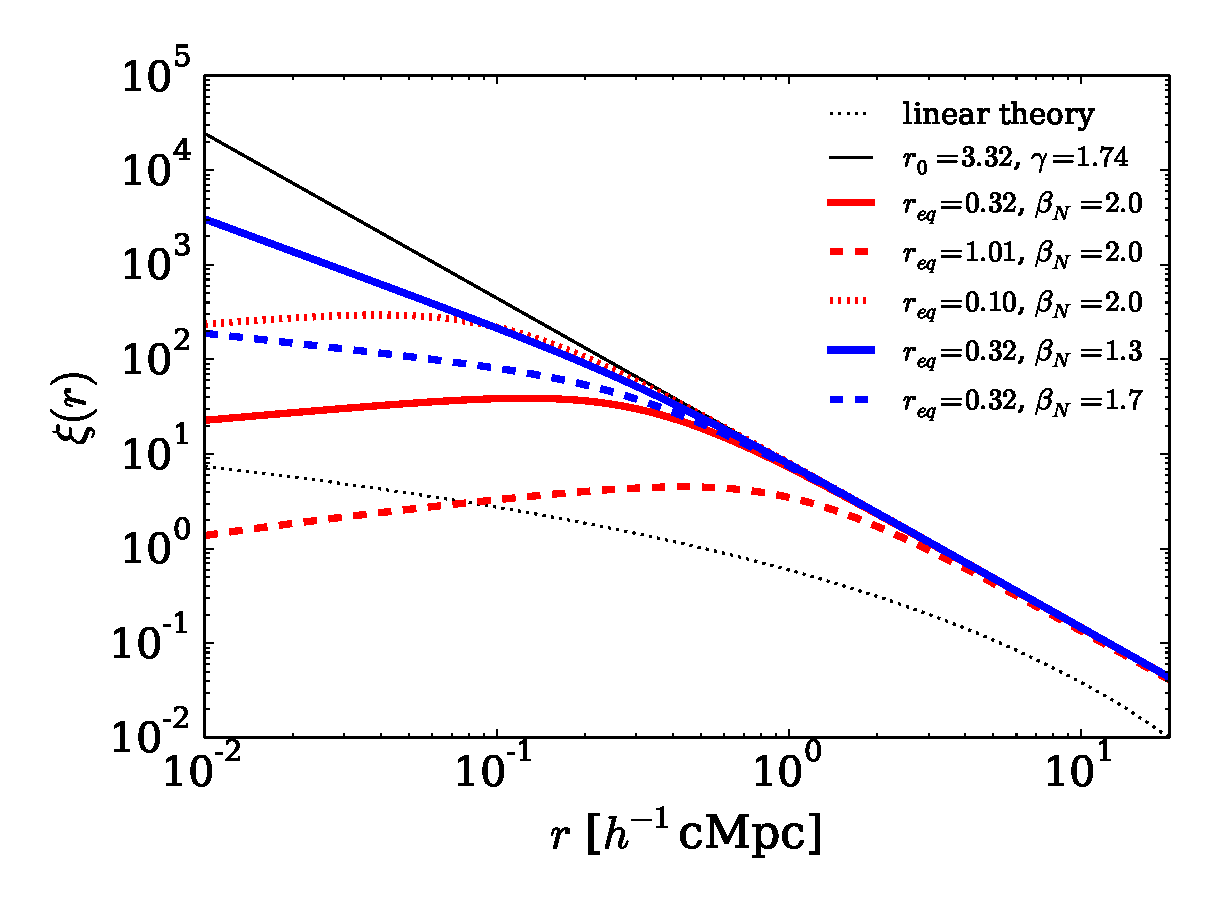
\includegraphics[angle=0,width=\columnwidth]{figure/corrfunc.pdf}
  \caption{The galaxy-absorber correlation function. The black line corresponds
    to the best-fit power-law LBG-DLA correlation function at $z\sim3$ by
    Cooke+(2006). The red and blue lines modify the Cooke+(2006) best-fit
    by inclusion of local photoionization effect. The red lines shows the 
    variation over the equality radius $r_{eq}$ and the blue lines shows the
    variation over the CDDF slope $\beta_N$.
    The turn-over of correlation function at
    small-scale only occurs when $\beta_N>\gamma/2+1$ is satified. 
    The equality radius is in the unit of $h^{-1}$cMpc.}
   \label{EoR_xi}
 \end{center}
\end{figure}


\subsubsection{The effect of reionization (or UV background fluctuation)}
Suppose a $\LyA$ forest-galaxy survey deeper towards the EoR. Toward the 
EoR, we expect some diffuse $\HI$ patches before the IGM engulfed by
the I-front. These $\HI$ patches in the QSO absorption spectra appears
as DLA-like feature (or LLS depending on $\HI$ column density). However,
in contrast to the ordinary LLS/DLAs around galaxies, the spatial position
is expected to be greater than the typical size of $\HII$ bubbles $r>R_b$. 
Therefore, in addition to post-reionized universe galaxy-absorber distribution
based on cosmic web, the correlation function on the scale $r>R_b$ will 
have extra contribution by the EoR-induced absorbers. (Just to illustrate
I plotted Fig.$\ref{EoR_xi}$. simplified version of McQuinn+2005 model).

While in practice we have only one $z\sim 7$ QSO, the availability of 
handful of $z\sim 6$ QSOs might allow us to measure this possible effect
towards the end of reionization. The existence of $\HI$ patch with increasing
correlation with galaxy on the scale $r>R_b$ will be a necessary diagnositic
criterion that we are appraoching to the EoR at $z>6$. However, it is worthwhile
to note the this may not be a sufficient condition because the UV background
fluctuation can produce additional correlation on the large-scale. 
Pontzen+(2014a,b) and Gontcho+(2014) have considered the effect of UV
background fluctuation on $\LyA$ forest correlation function and showed
the increase of correlation at large scale. Since the mean free path decrease
to higher redshift, the power can be added even on the scale compatible to
the $\HII$ bubble size. 

The existence of spikes on  $z\sim 6$ QSO absorption spectra provides the 
interesting oppotunity to apply galaxy survey in th $z\sim 6$ QSO fields.

\begin{figure}
 \begin{center}
  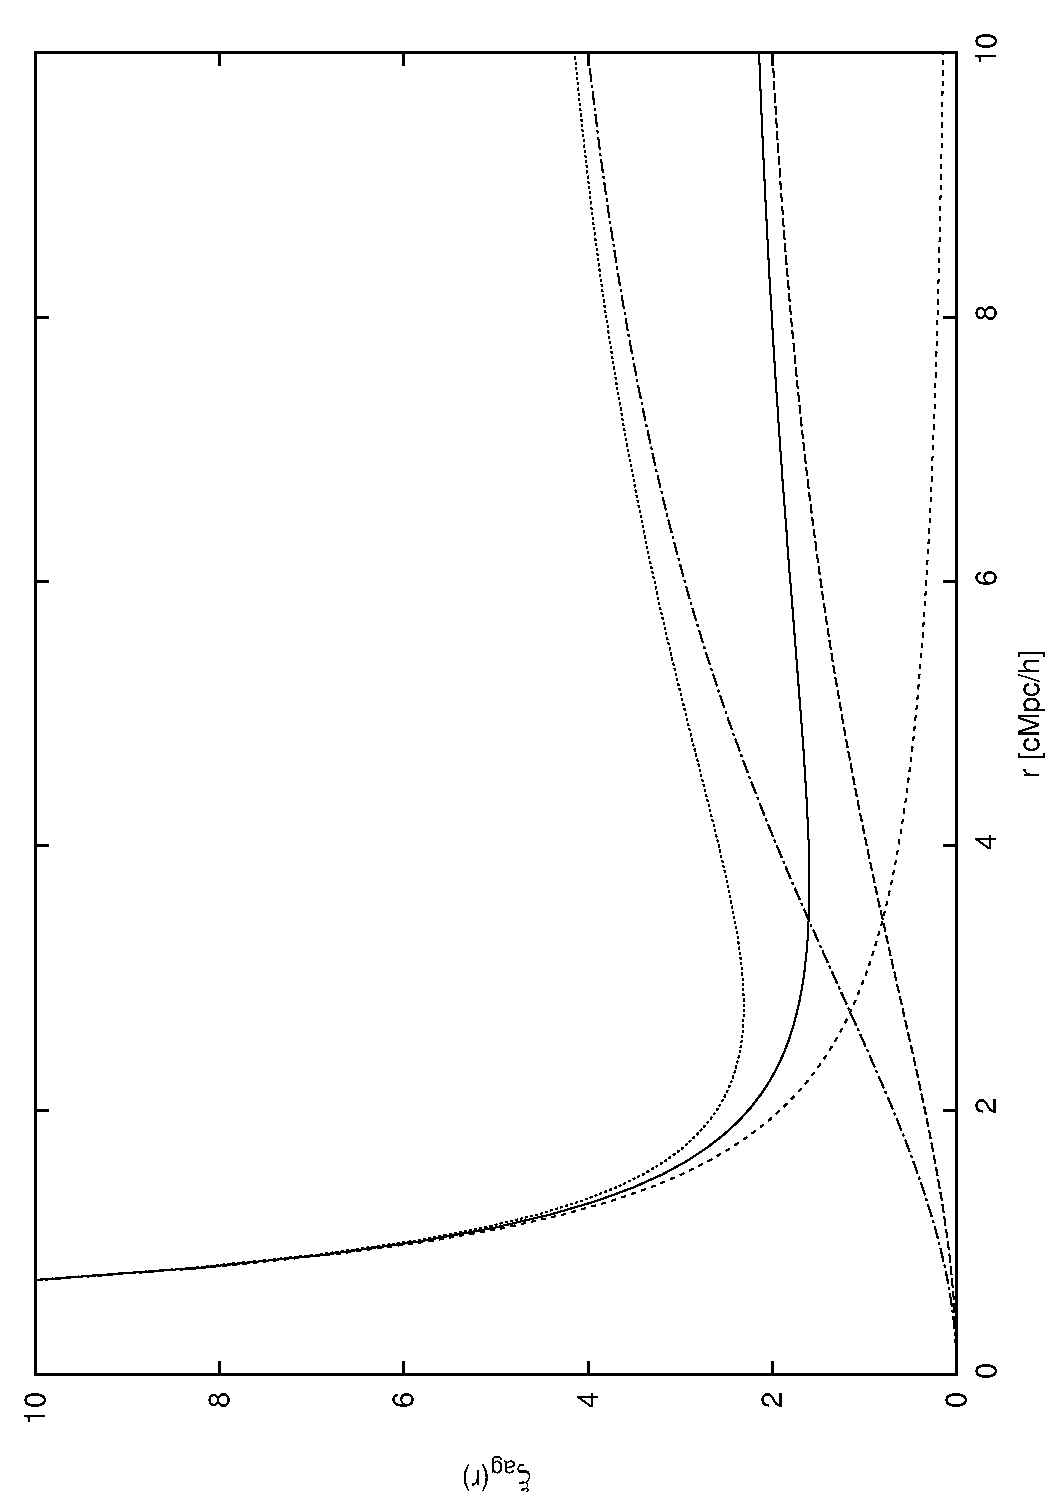
\includegraphics[angle=-90,width=\columnwidth]{figure/xi_example_EoR.pdf}
  \caption{galaxy-absorber correlation function. Illustrating example 
   effect of EoR. quick calc. just not to forget. 
   hyper-simplified model based on McQuinn+ 2005 \& Furlanetto+2004.
   \textbf{do this using simulation, then take a quick functional form here
   as a fitting function.}}
   \label{EoR_xi}
 \end{center}
\end{figure}



\subsubsection{Pairwise velocity statistics}


The conditional pairwise velocity distribution function $f(v_{12}|r_{12})$
at the fixed comoving seperation $r_{12}$ is followed from the rule of 
probability $f(v_{12},r_{12})=f(v_{12}|r_{12})f(r_{12})$. The mean pairwise velocity
is given by the first moment, $\langle v_{12}(r)\rangle=\int v_{12}f(v_{12}|r)
dv_{12}$. The pairwise velocity statistics is the central quantity in 
our formulation.


The streaming models require the modelling of the pairwise velocity statistics;
mean pairwise velocity $v_{12}(r)$ and pairwise velocity dispersion 
$\sigma_{12}^2(r,\mu)$. The BBGKY hierarchy provides a framework to relate the 
pairwise velocity statistics to the real-space clustering (Davis\&Peebles 1977;
Peebles 1980; Fry+; Hamilton 1988). Formally, the BBGKY hierarchy provides the
relation between velocity statistics such as pairwise streaming velocity
and velocity dispersion and N-point correlation function. 
We cast the traditional BBGKY hierarchy expressed in terms of dark matter or 
galaxies in the application to galaxy-absorber systems. The absorbers are the 
result of the IGM fluctuation in the cosmic web environment. 
We approximate the absorbers as a cloud. 
However in reality, $\LyA$ forest or self-shielded system, LLS/DLA, should be
viewed in terms of cosmic web. We mitigate this by considering the filaments or
walls of cosmic web as connection of clouds in a appropriate geometry. 

Suppose the phase-space distribution of galaxy and absorbers.
The first velocity moment of the BBGKY hierarchy expresses the
the conservation of pairs. This can more easily derived from the conservation
argument (Peebles 1976?; White's book). Suppose particles 
(galaxy-absorber pair) within a comoving radius $<r$ centred at a
particle, $N(<r,t)=\bar{n}(0)\int^r_0 4\pi r'^2dr'(1+\xi(r,t))$ where 
$\bar{n}(0)$ is the mean comoving number density (constant over redshift)
and $\xi(r,t)$ is the particle-particle (galaxy-absorber) correlation function.
The change in the total particle number $N(<r,t)$ is determined by the flux 
through the surface of sphere of radius $r$, which is 
$4\pi r^2\bar{n}(0)(1+\xi(r,t))\langle v_{12}\rangle$. Note that
$\langle v_{12}\rangle$ is the mean pairwise \textit{comoving} velocity.
\footnote{To avoid a confusion in various form appear in the literature,
proper velocity is $\langle v_{12}^{proper}\rangle=
a\langle v_{12}^{comoving}\rangle$.
\begin{equation}
\frac{\langle v_{12}^{proper}(r,a)\rangle}{Har}=-\frac{1}{1+\xi(r,a)}\frac{a}{r^3}
\frac{\partial}{\partial a}\int_0^r\xi(r',a)r'^2dr'
\end{equation}

 in the proper coordinates??,  
\begin{equation}
\frac{\partial \xi}{\partial t}+\frac{1}{r^2}
\frac{\partial}{\partial r}\left[r^2(1+\xi)\langle v_{12}(r,a)\rangle\right]=0
\end{equation}
}
We adopt the convention that the pairwise velocity is negative
for inflow and positive for outflow.

Thus, when the total number of particles are conserved,
\begin{equation}
\frac{\partial N}{\partial t}+
4\pi r^2\bar{n}(0)(1+\xi(r,t))\langle v_{12}\rangle=0
\end{equation}
By rearranging for $\langle v_{12}\rangle$, this follows the mean pairwise 
velocity field as (Davis\&Peebles 1977; Cooray \& Sheth 2002; White)
\begin{equation}
\langle v_{12}(r,t)\rangle=-\frac{1}{1+\xi(r,t)}\frac{1}{r^2}
\frac{\partial}{\partial t}\int_0^r\xi(r',t)r'^2dr'
\end{equation}

For linear theory, the correlation function scales as $\propto D(t)^2$,
the pairwise velocity field for unbiased tracer from the linear theory.
\begin{equation}
v_{12}(r)=-\frac{Hf(\Omega_m)}{\pi^2}\int P_L(k)j_1(kr) kdk
\end{equation}
where $f(\Omega)=d\ln D/d\ln a$.

For self-similar clustering,
\begin{equation}
v_{12}(r)=-\frac{v_{in}}{1+(r/r_0)^\gamma}
\end{equation}


\subsubsection{Pairwise velocity dispersion}

\begin{figure}
 \begin{center}
  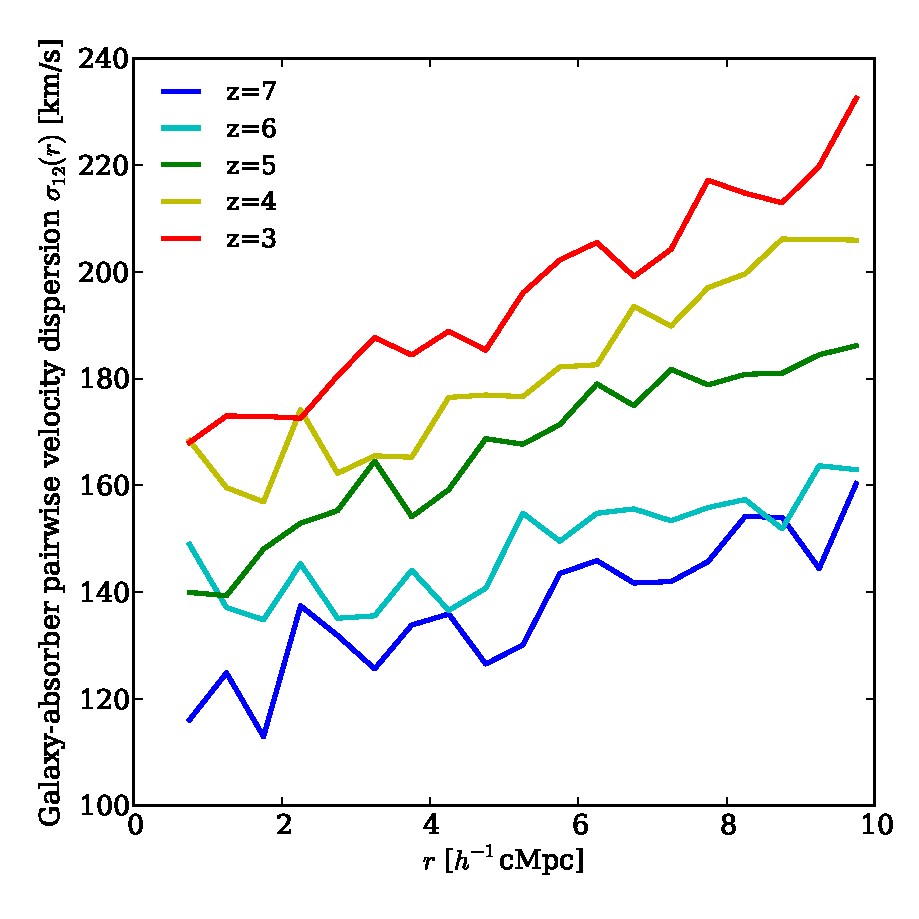
\includegraphics[angle=0,width=\columnwidth]{figure/s12_L40P256G256R0_Gamma12_SST.pdf}
  \caption{Radial pairwise velocity dispersion from simulation.}\label{s12}
 \end{center}
\end{figure}

The pairwise velocity dispersion is given by the second moment of 
BBGKY hierarchy, which depends on three-point correlation function.
The pairwise velocity dispersion has the contribution from (1)
the anisotropy of the absorber's velocity onto each central galaxies
(2) The dispersion among different galaxies' environment.
The former is, for example, the absorber accretion from filaments
is expected to have different velocity from the absorbers in
the direction of voids. The latter is caused by the fact that, 
even at the same radial pair seperation, the absorbers at different
central galaxies has the different pairwise velocity as they 
reside in the different part of cosmic web. 

The magnitude of this pairwise velocity dispersion is shown in Fig.\ref{s12}.
The pairwise velocity dispersion spans from about 100 to 250km/s.
The velocity dipsersion of galaxy-absorber pairs increase towards lower
redshift. This is a natural expectation from hiererchical structure formation.

While the simulation indicates the scale-dependece of pairwise velcoity
dispersion, for simplicity, we consider a constant pairwise velocity dispersion
to construct the joint model of redshift-space distortion and $\LyA$ RT.
Such assumption may introduce a bias on the inferred properties of
pairwise velocity field once the model is fitted to observations. 
These complications should be addressed by the mock observation
of simulations with expected observational errors. In this paper, we would
like to convey the framework that how the RSD of galaxy-absorber pairs
helps to understand $\LyA$ RT on the galaxy's visiblity. This would
aid to break the degenerarcy in the $\HI$ measurement in the EoR and 
$\LyA$ RT effect in cosmology with $\LyA$-emitting galaxies.

\subsubsection{Effect of feedback and outflow}
The feedback from galaxies is expected to modify the pairwise velocity
statistics. So far we have only considered the inflow which is purely
cosmological origin. What is the region of influence of feedbacks and
the outflow velocity?

From the observations of Steidel+ and Ouchi+, the velocity shift of
metal lines range from $v_{out}=100-600$km/s, which is believed to
be launched by some feedback mechanism. For the back-of-envelop
estimate of the region of influence of feedback, we consider a simple
mechanical kick of gas with velocity $v_{out}$ from a galaxy. To get
a rough upper estimate of the region of influence of feedback, ignore
the graviational force onto central galaxy. Then, during the age of 
a galaxy, say $t_{age}=1$Gyr, the inertial motion of gas can reach to
$v_{out}t_{age}\sim100-610$pkpc ($r_{\rm{infl}}\sim70-430(1+z)h_{70}^{-1}$ckpc), 
which is about the convensional definition of CGM ($<$300pkpc). 
The hydrodynamical simulation indicates the IGM properties beyond the
turn-around radius are well converged among different hydro scheme (SPH or
grid) and implemented feedback mechanisms (is there papers by Hopkins?, Schaye?,
Fumagalli?; Meiksin+2014).

Motivated by this argument, we consider a phenomenological model 
to include the outflow,
\begin{equation}
v_{12}(r)=2v_{out}e^{-r/r_{\rm{infl}}}-\frac{v_{in}}{1+(r/r_0)^\gamma}
\end{equation}

As a remark, any effect beyound the region of influence by `mechanical' 
feedback would only be possible by radiation field from galaxies. 
To influence the pairwise velocity of galaxy-absorber pairs we can
postulate either by energy-driven (radiative heating) or 
momentum-driven (radiation pressure). Note that the effect can be 
realized by the change of absorber abundance by the increased 
photoionziation rate by the local source as discussed in previous section.
Possible candiates for radiation pressure excerted on absorbers is
by $\LyA$ line, metal lines (for metal-enriched absorber) and dust 
(for dusty absorber). If these mechanism is in action, it is possible
to have a larger region of influce by radiation feedback.



\subsection{Redshift-space distortion}
The redshift-space distortion is the result of the line-of-sight pecular 
velocity between the tracers. For our interest, the tracers are galaxies 
(LAEs and LBGs) and absorbers ($\LyA$ forests and LLS/DLAs). 
The pairwise velocity between galaxies and absorbers imprint the redshift space
distortion signature. Turner? Rudie+? have measured the redshift space 
distortion consistent with coherent cosmological inflow for LBG samples. 

The mapping between redshift space and real space is
\begin{equation}
s_\perp=r_\perp,~~s_\parallel=r_\parallel+v_{12,\parallel}/H,
\end{equation}
The redshift-space correlation function $\xi_s(s_\parallel,s_\perp)$ can be 
modelled by the integration of real-space correlation function $\xi(r)$
with the pairwise velocity distribution function $f(v_{12,\parallel}|r)$ along a 
line-of-sight (Peeble 1980; Reid\&White (2006?); Fisher 1994-6?),
\begin{equation}
1+\xi_s(s_\parallel,s_\perp)=\int dv_{12,\parallel}f(v_{12,\parallel}|r)
\left[1+\xi(r)\right]
\end{equation}
where $r=\sqrt{s_\perp^2+(s_\parallel-v_{12,\parallel}/H)^2}$.
This is often referred to as streaming model (Peebles 1980; Jing+).

The central ingredient of the streaming model is the pairwise velocity
distribution $f(v_{12,\parallel}|r)$. Fisher (1995) has shown that the streaming
model with linear theory for $f(v_{12,\parallel}|r)$ is equivalent to the familar
Kaiser effect. Scoccimaro (2004) has shown that if pairwise velocity PDF is 
correct the streaming is valid for all scale (check the argument).


\subsection{Redshift-space correlation function}
Our aim is to develop a theory to interpret the observation of the 
galaxy-absorber correlation function in the redshift space. 
The redshit-space correlation function $\xi(s_\parallel,s_\perp)$ shows the 
anisotropy due to the redshift-space distortion imprinted by the peculiar 
velocity field. Although we do not intend to use such observations to measure 
$f=d\ln D/d\ln a$ as in modern LLS survey (e.g. BOSS, WiggleZ), we start with 
the linear theory to build up a solid understanding.


The two-dimensional correlation function is usually expanded in Legendre
Polynomials $L_\ell(\mu_s)$ where $\mu_s=s_\parallel/s$ (Reid\&White, Reid+2012;
Hamilton 1992),
\begin{equation}
\xi(s,\mu_s)=\sum_{\ell=0}^\infty\xi_\ell(s)L_\ell(\mu_s),
\end{equation}
where
\begin{equation}
\xi_\ell(s)=\frac{2\ell+1}{2}\int d\mu_s \xi(s,\mu_s)L_\ell(\mu_s).
\end{equation}
For large-scale structure studies, the first three even Legendre moments
$\xi_0(s)$, $\xi_2(s)$ and $\xi_4(s)$ are usually considered. 
The quadrupole-monopole ratio $\xi_2/\xi_0$ is positive for streching
in radial direction and negative for flattening. Coherent inflow produce
the negative quadrupole-monopole ratio, while random velocity dispersion
and coherent outflow give positive value.


In linear theory, Kaiser formula translates to (Hamilton 1992; Reid\&White 2011)
\begin{equation}
\xi_\ell(s)=i^\ell\int\frac{dk}{k}\Delta^2_\ell(k)j_\ell(ks),
\end{equation}
where 
\begin{eqnarray}
\Delta^2_0(k)&=&\Delta^2_{L}(k)(b^2+\frac{2}{3}bf+\frac{1}{5}f^2), \\
\Delta^2_2(k)&=&\Delta^2_{L}(k)(\frac{4}{3}bf+\frac{4}{7}f^2), \\
\Delta^2_4(k)&=&\Delta^2_{L}(k)(\frac{8}{35}f^2),
\end{eqnarray}





\subsubsection{Pairwise velocity PDF}
For the perfectly coherent velocity field, 
\begin{equation}
1+\xi^s(s_\parallel,s_\perp)=\int dr_\parallel
\left[1+\xi(\sqrt{s^2_\perp+r_\parallel^2})\right]
\delta_D\left[s_\parallel-r_\parallel-\mu v_{12}(r)\right]
\end{equation}
where $r=\sqrt{r_\perp^2+r_\parallel^2}$ and $\mu=r_\parallel/r$. 
The redshift-space correlation function is then given by
$\xi^s(s_\parallel,s_\perp)=\xi(\sqrt{s^2_\perp+r_\parallel^2(s_\parallel)})$
where $r_\parallel(s_\parallel)$ is the solution of implicit equation
$s_\parallel=r_\parallel\left(1-\frac{v_{12}(r)}
{r}\right)$.

By assuming the velocity PDF is gaussian,
we arrive at the Gaussian streaming model (Reid\&White 2011)
\begin{eqnarray}
&&1+\xi^s(s_\parallel,s_\perp)=\int \frac{dy}{\sqrt{2\pi\sigma_{12}^2(r,\mu)}}\times
 \\
&&~~~~~~~\left[1+\xi(\sqrt{s^2_\parallel+y^2})\right]
\exp\left[-\frac{(s_\parallel-y-\mu v_{12}(r))^2}{2\sigma^2_{12}(r,\mu)}\right]
\nonumber
\end{eqnarray}




\section{Theory: The environmental dependence of $\LyA$ visibility}



\subsection{Cosmological $\LyA$ radiative transfer}
The statitical formulation of the $\LyA$ raditive transfer can start
with Paresce, McKee Bowyer 1980. The critical difference between continuum
RT and line RT is that the former is sentitive to the clustering in real
space whereas the latter is to in \textit{velocity space}. For $\LyA$ RT
what matters is where the absorber occupies in the velocity space (marginalised
over real space position).
The probability of an absorbering cloud's velocity within $v$ and $v+dv$
is $p(v)dv$. Then the probability that a line-of-sight of $\LyA$ galaxy to 
the observer does not coincide is $[1-p(v)]dv$. The fraction of photons absorbed
is $p(v)e^{-\tau(v)}dv$
\begin{equation}
\langle I(v+\Delta v)\rangle=\langle I(v)\rangle
\left\{
(1-p(v))\Delta v+p(v)e^{-\tau(v)}\Delta v
\right\}
\end{equation}
Forming the differential equation by $d\langle I\rangle/dv\approx
\langle I\rangle[p(v)(1-e^{-\tau(v)})]$, whose solution is
$\langle I\rangle=\langle I\rangle_0e^{-\tau_{\rm{eff}}}$
\begin{equation}
\tau_{\rm{eff}}=\int_{-\infty}^\infty p(v_{12})\left[1-e^{-\tau(v_{12})}\right]dv_{12}
\end{equation}
where $v_{12}$ is the pairwise velocity of absorber and galaxy.

The pairwise velocity PDF $p(v_{12})$. Maybe an approach is cumulant
expansion with respect to N-point correlation function derived from 
BBGKY hierarchy. The truncate with 2PCF (see Scherrer \& Bertschinger 1991)? 
From the Bayes' rule 
\begin{equation}
p(v_{12})=\int p(v_{12}|r)p(r)dr
\end{equation}
where $p(r)dr=\frac{4\pi r^2}{V}(1+\xi(r))dr$ is the PDF from the 
real-space clustering of absorber around galaxy.

The end result for Gaussian pairwise velocity PDF.
\begin{equation}
\tau_{\rm{eff}}=\int d\NHI\frac{d\mathcal{N}}{d\NHI}
\int dv p(v_{12})\left[1-e^{-\tau(v_{12},\NHI)}\right]
\end{equation}
\begin{equation}
p(v_{12})=\int \frac{d^3r}{\sqrt{2\pi\sigma_{12}^2(\boldsymbol{r})}}
\left(1+\xi(\boldsymbol{r})\right)
\exp\left[\frac{(v_{12}-\langle v_{12}(\boldsymbol{r})\rangle)^2}
{2\sigma_{12}^2(\boldsymbol{r})}\right]
\end{equation}

Pairwise velocity at $\boldsymbol{r}$ is $v_{12}(\boldsymbol{r})$.
$\xi_v(\boldsymbol{r})=\langle v_{12}(\boldsymbol{x})
v_{12}(\boldsymbol{x}+\boldsymbol{r})\rangle$

We can imagine two models, dirac delta PDF $p(v_{12}|r)=\delta_D(v_{12}-aHr)$






\subsection{The region of influence}
For both EoR $z>6$ (McQuinn+; Dikjstra+) and the post-reionized universe 
$2<z<6$ (Zheng+; Dijkstra\&Wyithe), the IGM environment influence the
visibility of $\LyA$-emitting galaxies. The degree of the impact depends
on the amount of clustering of gas, velocity field, and photoionization
background in the vicinity of the galaxies. The $\LyA$ radiative transfer
is sensitive to the velocity structure. The gas velocity field is nonlinear
in and out of galactic haloes, but at large enough distance it would 
converge to Hubble flow. The region of influence of $\LyA$ RT is most 
directly characterized in the velocity space. The wing approximation to
the Lorentz profile $\varphi_\nu=\frac{\Lambda/4\pi^2}{(\nu-\nu_\alpha)^2+(\Lambda/4\pi)^2)}
\approx\frac{\Lambda}{4\pi^2(\nu-\nu_\alpha)^2}$ where $\Lambda=6.25\times10^8s^{-1}$ is
the damping coefficient.  The optical depth of 
an absorber of column density $\NHI$ and total (hubble flow plus peculiar)
proper velocity $v_c$ is $\tau_\alpha(\nu_e)=\sigma_\alpha\NHI\varphi_\nu[\nu_e(1-v_c/c)]$
The absorber velocity that gives the optical depth $\tau_\alpha$
against $\LyA$ line emission from galaxies is 
\begin{equation}
v_c(\tau_\alpha)=c\sqrt{\frac{\sigma_\alpha\NHI\Lambda}{4\pi^2\nu_\alpha^2\tau_\alpha}}
=507.3\tau_\alpha^{-1/2}\left(\frac{\NHI}{10^{20}cm^2}\right)^{1/2}\rm{km/s}
\end{equation}
For a strong absorbing cloud to give the optical depth of unity (37\% transmission) 
against the $\LyA$ line emission, the absorbing cloud cannot be 
outflowing relative to the central galaxy more than $\sim500-2800\rm{km/s}$.
This defines the region of influence of $\LyA$ RT in the velocity space.
To translate the region of influence to the real space we need to know the
velocity field around a galaxy. For pure Hubble flow the comoving region of influence
is 
\begin{equation}
D_{\rm{infl}}=\frac{v_c(\tau_\alpha)}{H_0}\frac{1+z}{[\Omega_m(1+z)^3+\Omega_\Lambda]^{1/2}}
\end{equation}
\subsection{Statistical formulation}
The statitical formulation of the $\LyA$ raditive transfer can start
with Paresce, McKee Bowyer 1980. An alternative derivation, which clarifies 
the implicit assumptions and allow generalization, is shown in Appendix.
The critical difference between continuum
RT and line RT is that the former is sentitive to the clustering in real
space whereas the latter is to in \textit{velocity space}.
The probability of an absorbering cloud's velocity within $v$ and $v+dv$
is $p(v)dv$. Then the probability that a line-of-sight of $\LyA$ galaxy to 
the observer does not coincide is $1-p(v)dv$. The fraction of photons absorbed
is $p(v)e^{-\tau(v)}dv$
\begin{equation}
\langle I(v+\Delta v)\rangle=\langle I(v)\rangle
\left\{
(1-p(v)\Delta v)+p(v)e^{-\tau(v)}\Delta v
\right\}
\end{equation}
Forming the differential equation by $d\langle I\rangle/dv\approx
\langle I\rangle[p(v)(1-e^{-\tau(v)})]$, whose solution is
$\langle I\rangle=\langle I\rangle_0e^{-\tau_{\rm{eff}}}$
\begin{equation}
\tau_{\rm{eff}}=\int_{-\infty}^\infty p(v_{12})\left[1-e^{-\tau(v_{12})}\right]dv_{12}
\end{equation}
where $v_{12}^{tot}=aHr_{12}+v_{12}$ is the \textit{total, proper pairwise 
velocity} of absorber and galaxy. By transforming the variables $r_{12}, v_{12}$
into $v_{12}^{tot}$,
\begin{eqnarray}
f(v_{12}^{tot})&=&\iint\delta_D\left[v_{12}^{tot}-(Hr_{12}+v_{12})\right]
f(v_{12},r_{12})dv_{12}dr_{12} \nonumber \\
&=&\int f(v_{12}^{tot}-Hr_{12}|r_{12})f(r_{12})dr_{12}
\end{eqnarray}
where $f(r)dr=\frac{4\pi r^2}{V}(1+\xi(r))dr (NO!)$ 
CORRECT ONE is $f(r)dr=\frac{1}{L}(1+\xi(r))dr$ (pre-factor
dendendence is geometric factor for 1D along a skewer it does not enter!)
is the PDF from the 
real-space clustering of absorber around galaxy.

total velocity $v_\parallel^{tot}=H s_\parallel=H(r_\parallel+v_\parallel/H)$
\begin{equation}
I(s+ds)=I(s)\left\{1-p(s_\parallel,\NHI)ds_\parallel+p(s_\parallel,\NHI)
e^{-\tau(s_\parallel,\NHI)}ds\right\}
\end{equation}


The end result for Gaussian pairwise velocity PDF.

\begin{equation}
\tau_{\rm{eff}}=\int d\NHI\frac{\partial^2\mathcal{N}}{\partial\NHI\partial z}
\left|\frac{dz}{dr}\right|
\int dv f(v_{12})\left[1-e^{-\tau(v_{12},\NHI)}\right]
\end{equation}
\begin{equation}
f(v_{12})=\int \frac{dr}{\sqrt{2\pi\sigma_{12}^2(r)}}
\left(1+\xi(r)\right)
\exp\left[\frac{(v_{12}^{tot}-Hr-\langle v_{12}(r)\rangle)^2}
{2\sigma_{12}^2(r)}\right]
\end{equation}



The end result for Gaussian pairwise velocity PDF.
\begin{equation}
\tau_{\rm{eff}}=\int d\NHI\frac{d\mathcal{N}}{d\NHI}
\int dv f(v_{12})\left[1-e^{-\tau(v_{12},\NHI)}\right]
\end{equation}
\begin{equation}
f(v_{12})=\int \frac{4\pi r^2dr}{\sqrt{2\pi\sigma_{12}^2(r)}V}
\left(1+\xi(r)\right)
\exp\left[\frac{(v_{12}^{tot}-Hr-\langle v_{12}(r)\rangle)^2}
{2\sigma_{12}^2(r)}\right]
\end{equation}


The end result for Gaussian pairwise velocity PDF.
\begin{equation}
\tau_{\rm{eff}}=\int d\NHI\frac{d\mathcal{N}}{d\NHI}
\int dv f(v_{12})\left[1-e^{-\tau(v_{12},\NHI)}\right]
\end{equation}
\begin{equation}
f(v_{12})=\int \frac{4\pi r^2dr}{\sqrt{2\pi\sigma_{12}^2(r)}V}
\left(1+\xi(r)\right)
\exp\left[\frac{(v_{12}^{tot}-Hr-\langle v_{12}(r)\rangle)^2}
{2\sigma_{12}^2(r)}\right]
\end{equation}

For generalization to the anisotropic real-space clustering, e.g.
biconical outflow + two cold streaming model
\begin{equation}
f(v_{12})=\int \frac{d^3r}{\sqrt{2\pi\sigma_{12}^2(\boldsymbol{r})}}
\left(1+\xi(\boldsymbol{r})\right)
\exp\left[\frac{(v_{12}-\langle v_{12}(\boldsymbol{r})\rangle)^2}
{2\sigma_{12}^2(\boldsymbol{r})}\right]
\end{equation}

Pairwise velocity at $\boldsymbol{r}$ is $v_{12}(\boldsymbol{r})$.
$\xi_v(\boldsymbol{r})=\langle v_{12}(\boldsymbol{x})
v_{12}(\boldsymbol{x}+\boldsymbol{r})\rangle$

We can imagine two models, dirac delta PDF $p(v_{12}|r)=\delta_D(v_{12}-aHr)$


\begin{figure*}
 \begin{center}
  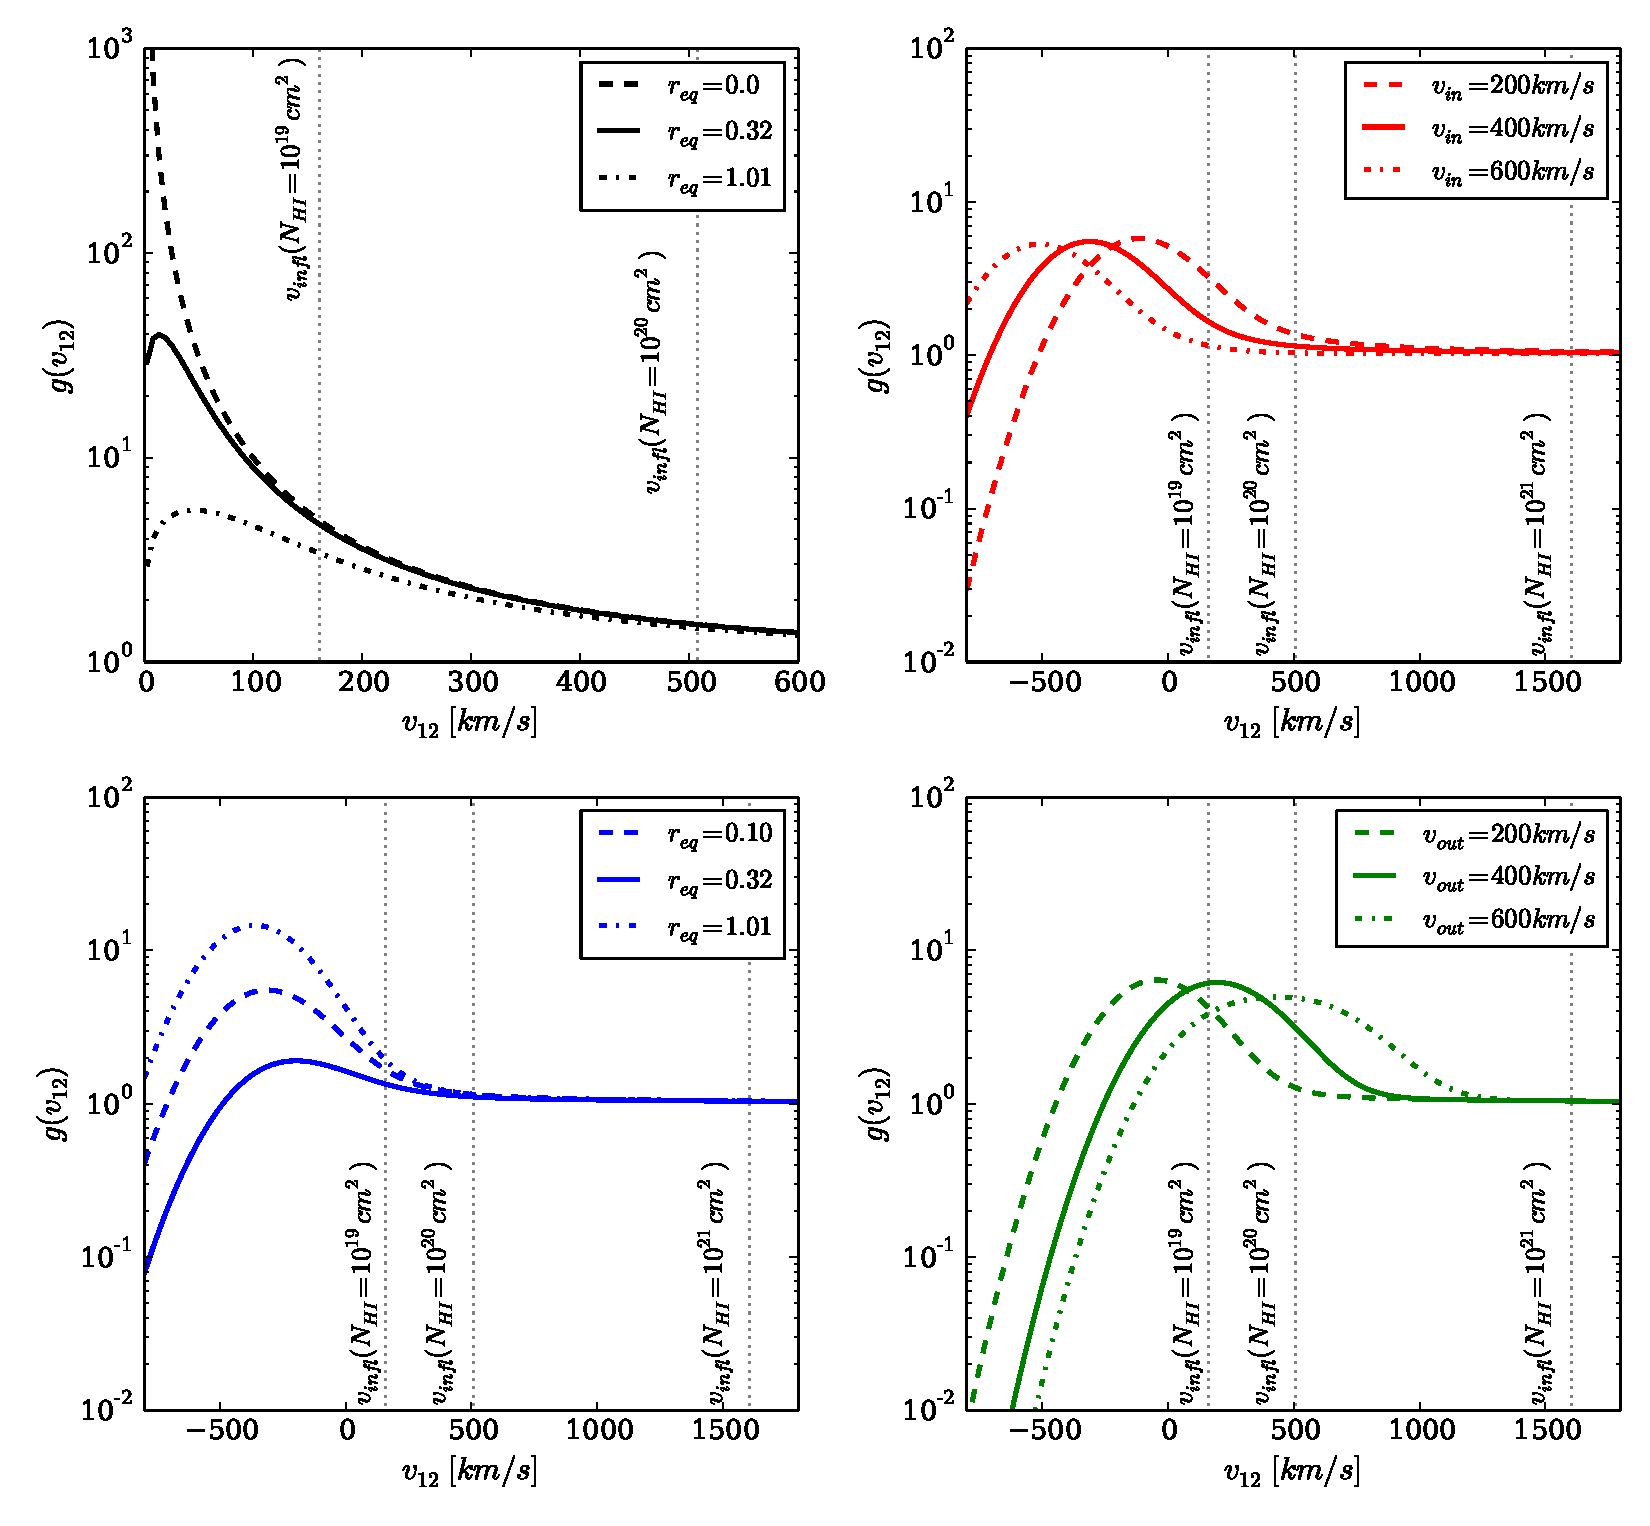
\includegraphics[angle=0,width=0.7\textwidth]{figure/v12_distribution.pdf}
  \caption{pairwise velocity distribution. Enhancement due to velocity space
  clustering}
 \end{center}
\end{figure*}

\begin{figure}
 \begin{center}
  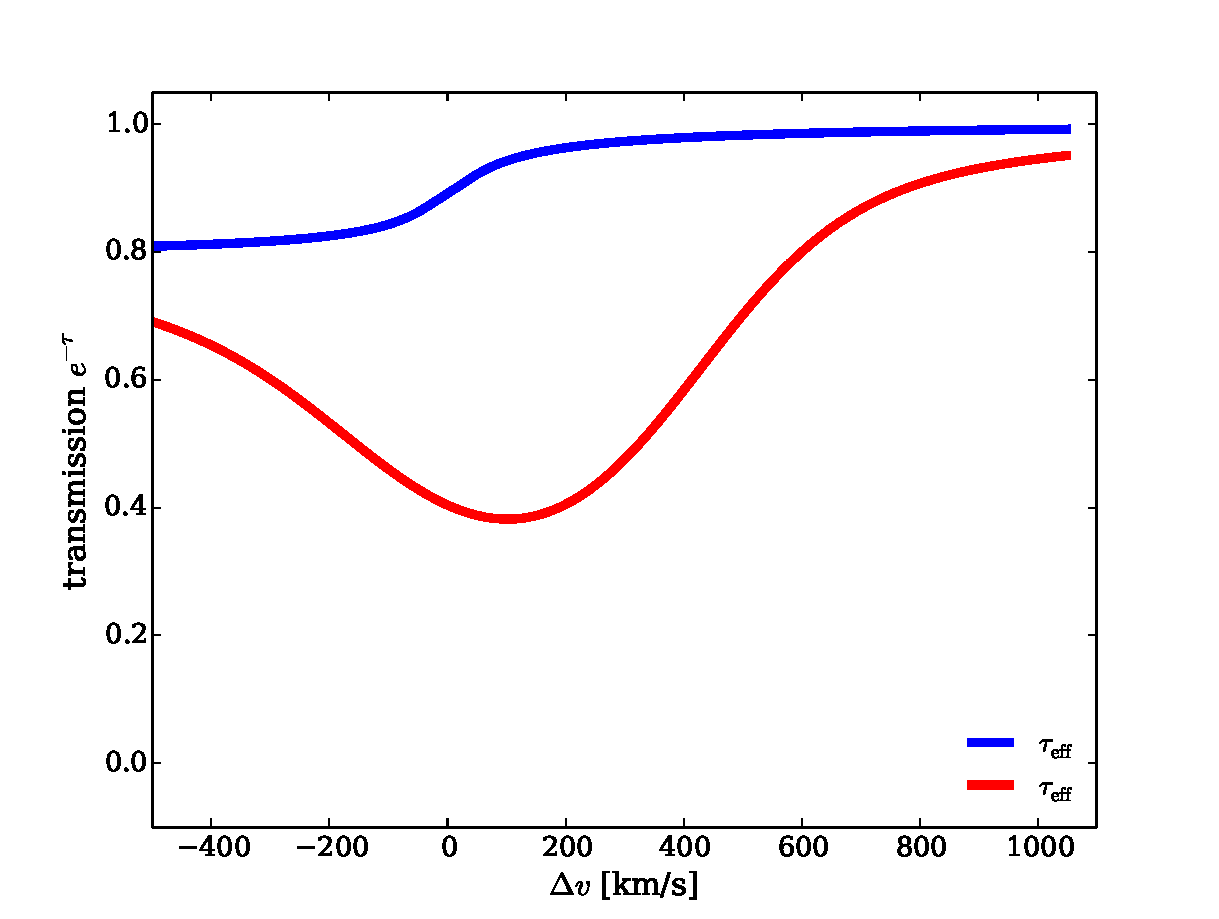
\includegraphics[angle=0,width=\columnwidth]{figure/test_eff_optdpt.pdf}
  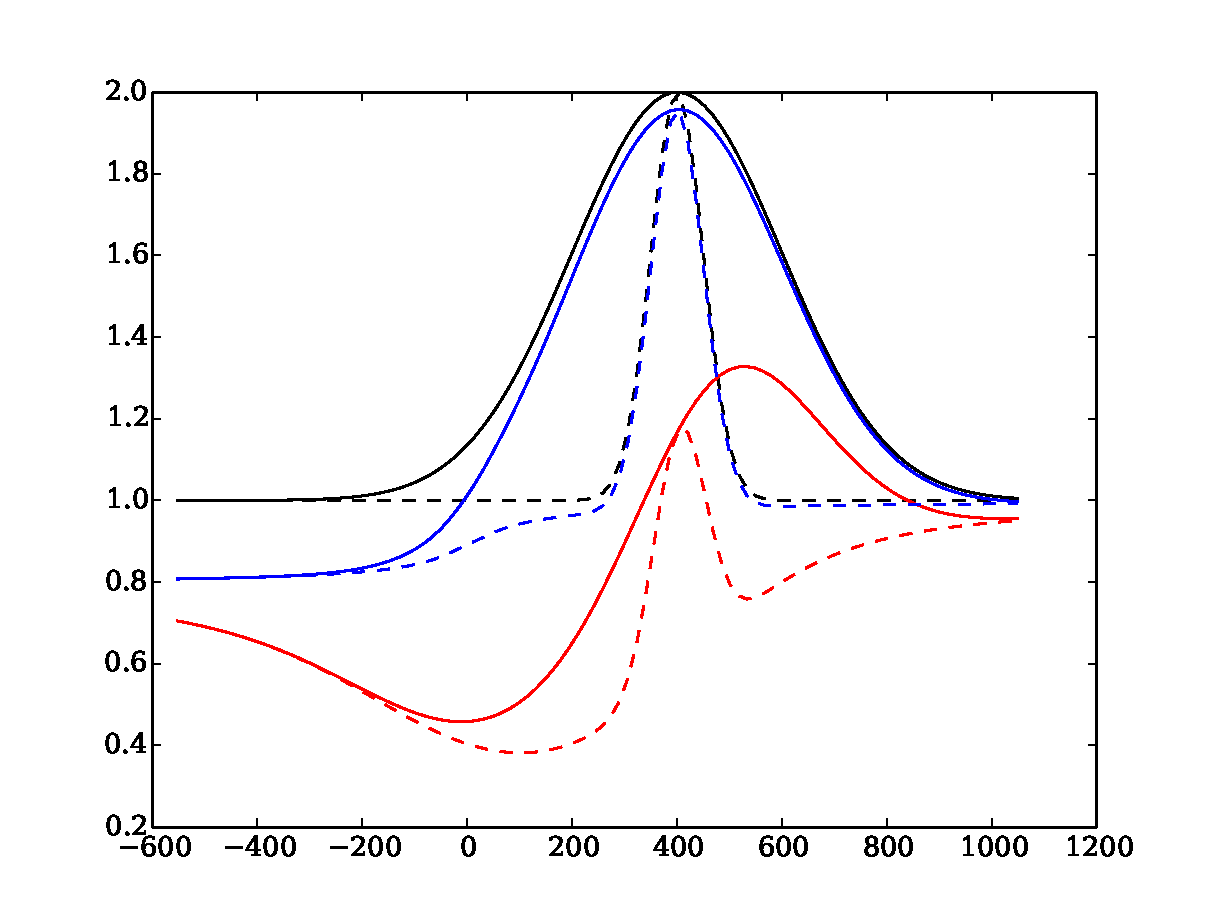
\includegraphics[angle=0,width=\columnwidth]{figure/test_lya_profile.pdf}
  \caption{Example calc. of effective optical depth with statistical formalism}
 \end{center}
\end{figure}



\subsection{Caveats}
\subsubsection{Pairwise velocity PDF}
How good is the gaussian approximation to pairwise velocity PDF? The assumption
that the pairwise velocity PDF may introduce systematic bias in analytic model.
Scoccimaro 2004 has studied that the pairwise velocity PDF is in fact highly
non-gaussian with skewness and kurtosis. Tinker 2005? modelled the non-gaussian
pairwise velocity PDF in the HOD framework. Generalisation can also be done
possibly by the cumulant expansion or Edgeworth expansion 
(e.g. Matsubara2008+; Sherrer\&Bertschinger 1991).

Scoccimaro 2004 argued that the direct recontruction of the PDF from 
redshift-space clustering measurement is in general impossible, which
must rely on the assumption of scale-independent PDF or Gaussianity.


The pairwise velocity PDF $p(v_{12})$. Maybe an approach is cumulant
expansion with respect to N-point correlation function derived from 
BBGKY hierarchy. The truncate with 2PCF (see Scherrer \& Bertschinger 1991)? 


\section{Application of theory}
\subsection{Spectral synthesis with the intergalactic environment}

We show an application of the joint model of RSD and $\LyA$ RT to
the stellar population synthesis. 
We have been considering the deep spectroscopic galaxy survey in the 
foreground of QSOs. The availability of spectroscopy of individual 
galaxies were supposed to perform the RSD measurement. 

The statistical formalism presented in the section 3 allows us to perform
the spectral synthesis including the RT effect of large-scale environment.
Since the independent constraint on $\LyA$ effective optical depth can
be provided from the RSD measurement. 

The distribution of foregound absorbers of the galaxies attenuates
the restframe wavelength shorther than $1216\rm{\AA}$ by Lyman series 
line blancketing and photonionization absorption ($<912$\AA)
(Madau 95, Meiksin 06, Inoue 12). 

\begin{figure*}
 \begin{center}
  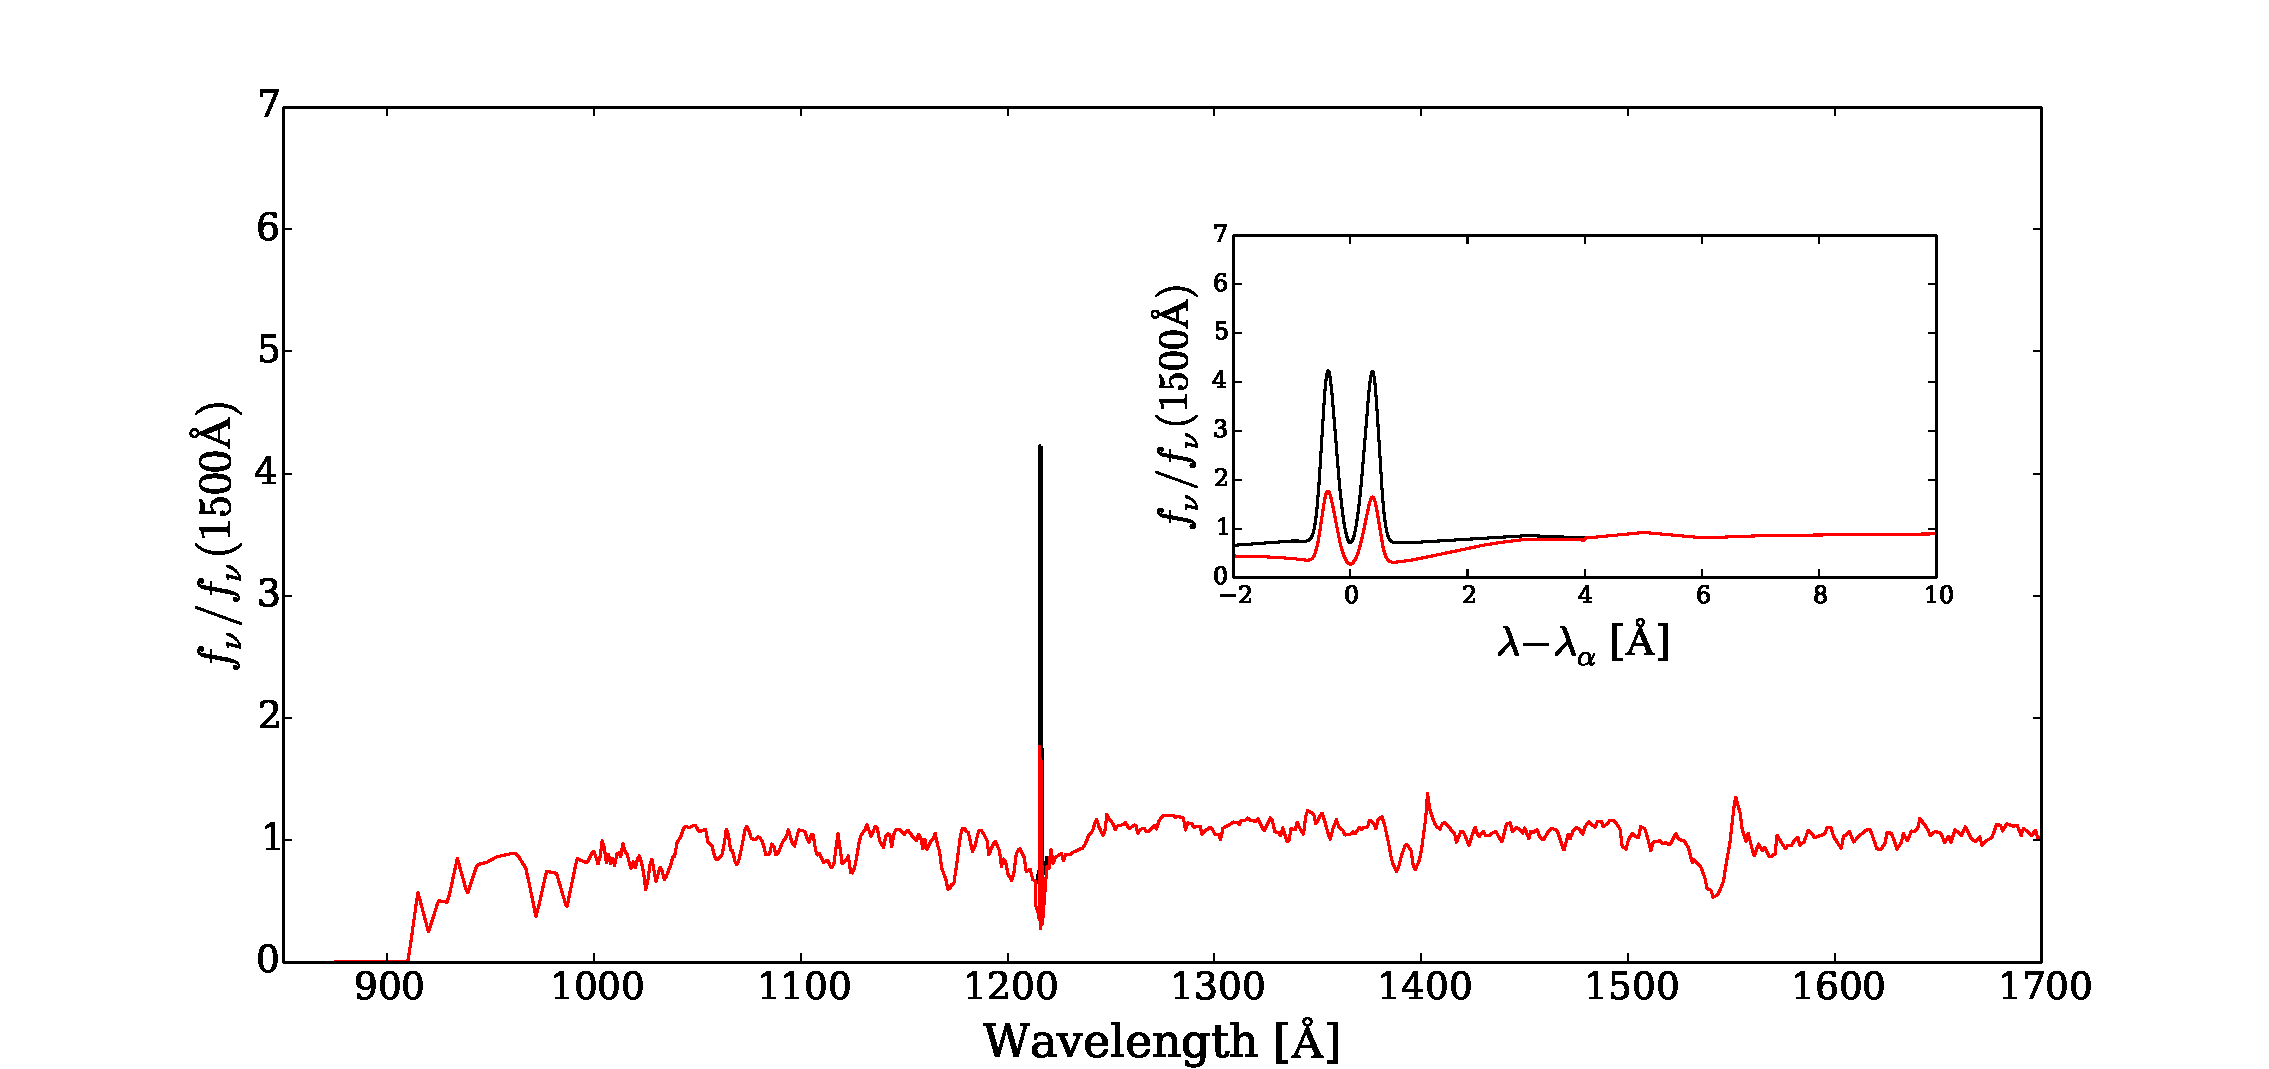
\includegraphics[angle=0,width=\textwidth]{figure/spectral_synthesis.pdf}
  \caption{example spectral synthesis.}
 \end{center}
\end{figure*}

\begin{figure}
 \begin{center}
  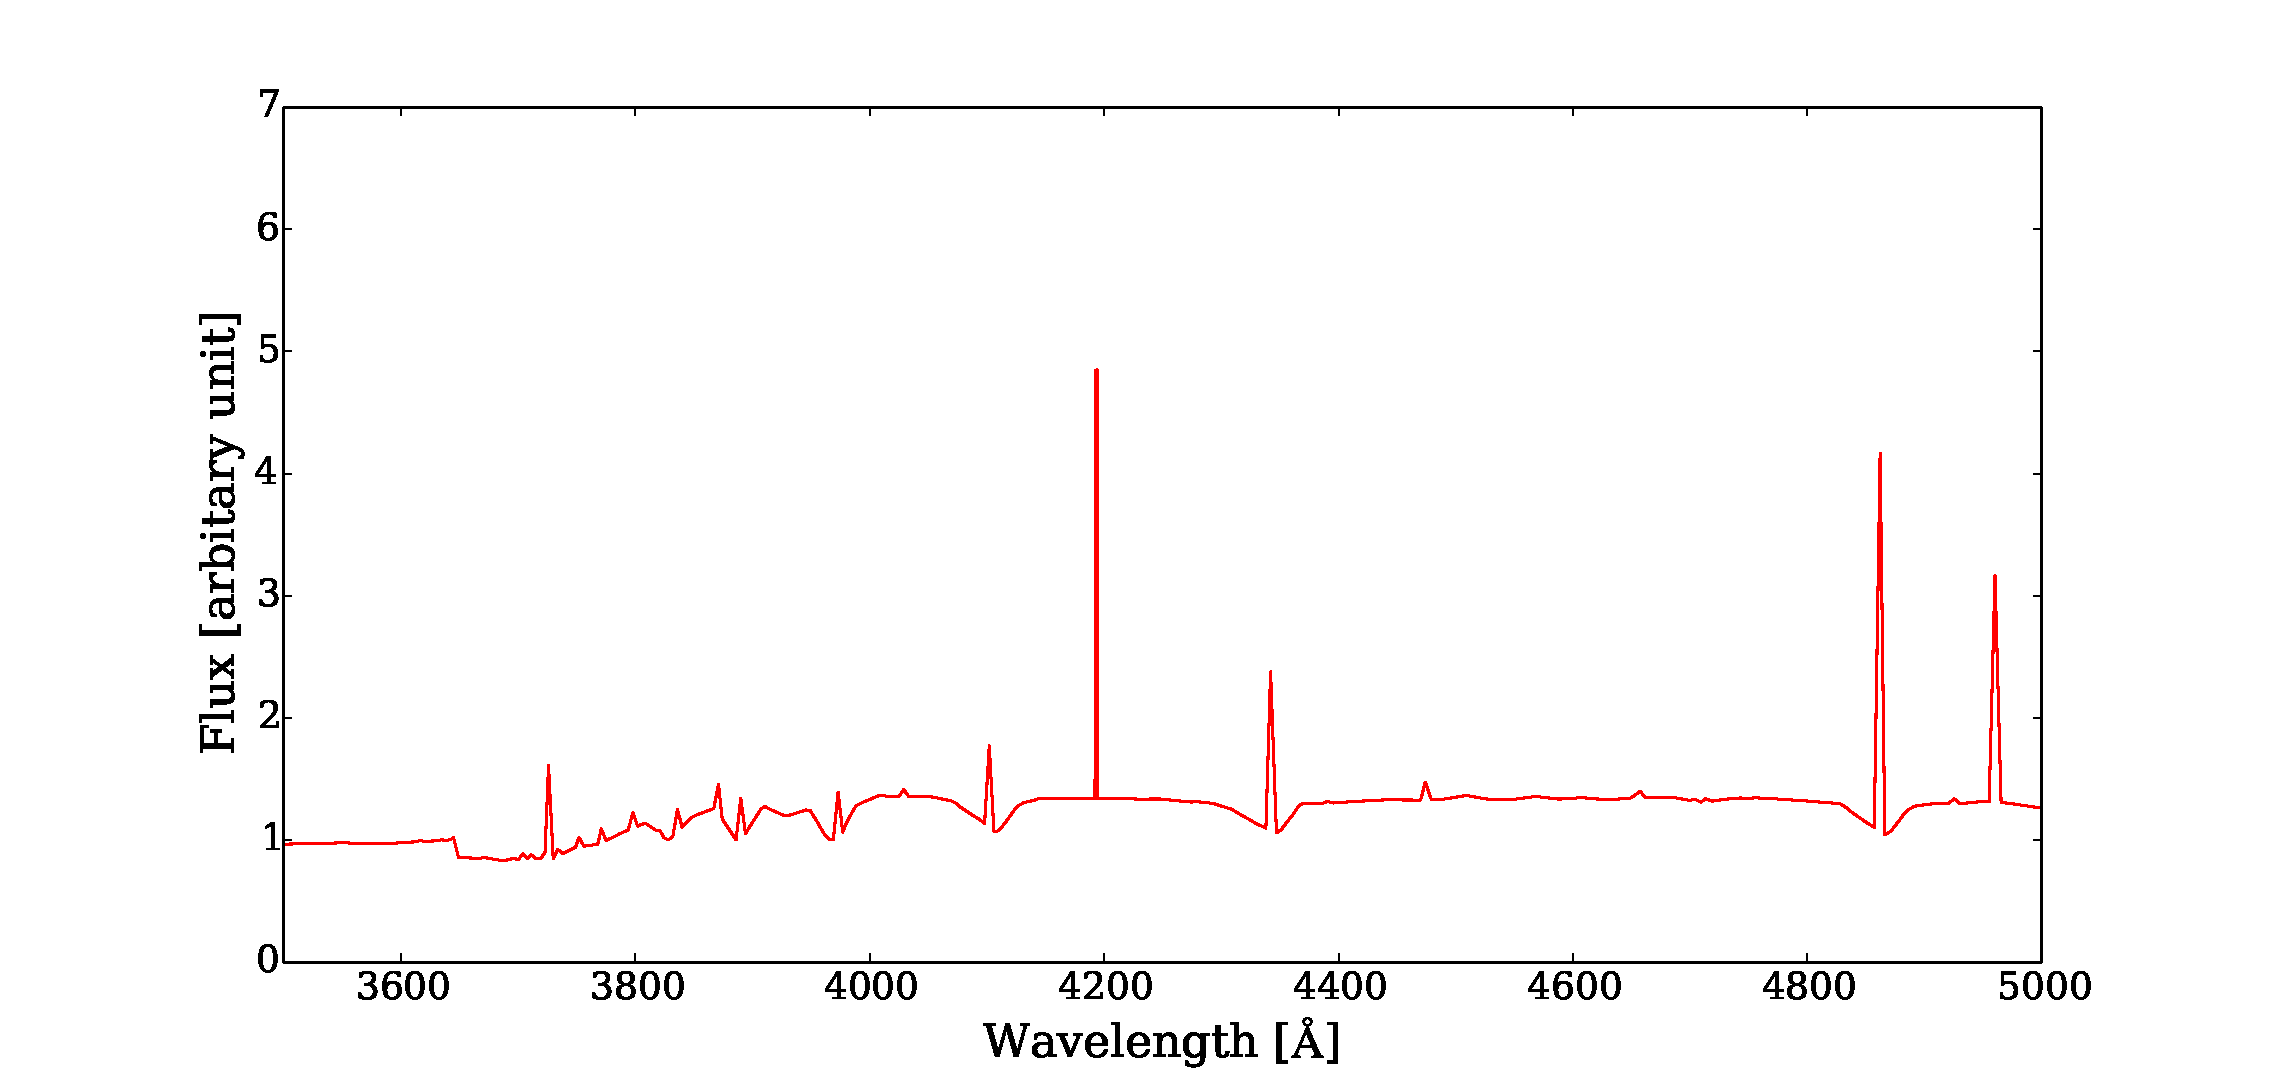
\includegraphics[angle=0,width=\columnwidth]{figure/spectral_synthesis_3500-5000.pdf}
  \caption{Optical part of synthetic spectrum.}
 \end{center}
\end{figure}



\section{Simulation}
\subsection{Cosmological hydrodynamical simulation}

\begin{table*}
\centering
\caption{Simulation set up}
\label{table:ramses}
\begin{tabular}{llllllllll}
\hline
name        & Box size $L$       & $N_{\rm{DM}}$ & $N_{\rm{grid}}(base)$ &  $N_{\rm{grid}}(fine)$   & $m_{\rm{DM}}$          &$\Delta L(base)$ & $\Delta L(fine)$  & $z_{ini}$ & $J_{21}, \alpha, z_{reion}$ \\ 
            & [$h^{-1}\rm{cMpc}$] &             &                    &                       & [$h^{-1}\rm{M}_\odot$] &[$h^{-1}\rm{ckpc}$] &             \\
\hline
\multicolumn{2}{l}{\underline{static grid + adiabatic}} \\
L10P256G256R0 &  10              & $256^3$   & $256^3$     &     & $3.57\times10^6$      & 39.1       &        & 276  \\
L20P256G256R0 &  20              & $256^3$   & $256^3$     &    & $2.86\times10^7$      & 78.1        &       & 237   \\
L40P256G256R0 &  40              & $256^3$   & $256^3$     &    & $2.29\times10^8$      & 156.2       &       & 199   \\
L60P256G256R0 &  60              & $256^3$   & $256^3$     &    & $7.72\times10^8$      & 234.4       &       &  178   \\
\multicolumn{2}{l}{\underline{AMR grid + adiabatic}} \\
L40P256G256R2 &  40              & $256^3$   & $256^3$     & $1024^3$   & $2.29\times10^8$      & 156.2      &  39.1      & 199   \\
\multicolumn{2}{l}{\underline{static grid run + UV background}} \\
L40P256G256R0 &  40              & $256^3$   & $256^3$     &    & $2.29\times10^8$      & 156.2       &       & 199   & 1.0, 1.0, 8.5 \\


\hline
\end{tabular}

\end{table*}

We carried out the cosmological hydrodynamical simulation of the IGM using 
AMR hydro/$N$-body code RAMSES (Teyssier 2002). We performed a series of 
adiabatic simulation with varying box size and resolution elements for 
convergence test. 

We adopt the quasi-Lagrangian refinement strategy with refinement criterion 
of 10 particles by which the cell is refined when the number of dark matter 
particle or equivalent gas mass exceeds 10.  

The initial condition is generated with COSMICS package (Bertschinger 1996?). 
The COSMICS package is initialized by setting the initial rms fluctuation 
$\sigma_8(z=z_{ini})=0.03$. Because the resolution of simulations are varying 
the initial redshift is elevated to lower redshift for lower resolution 
simulation. The initial temperature is set as $T=650\rm{K}$.This is compromise 
because the adiabatic simulation does not include Compton heating from CMB and 
cooling. The IGM only be cooled or heated by adiabatic process.

The haloes are identified by HOP algorithm (Eisenstein+; Aubert).

\subsection{Radiative transfer}
We introduce the self-shielded gas by Rhamati+ criterion. The method
is calibrated based on radiative transfer simulation.

\subsection{Synthetic QSO spectra}

\subsection{Synthetic galaxy catalogue}


\section{survey: mock}






\section{Results}
\subsection{Dynamics of galaxy-absorber pairs}
To build the understanding of the dynamics of large-scale environment
of galaxies, i.e. galaxy-absorber pairs, we compare the 
analytic models (linear theory and self-similar ansatz) with 
numerical simulation.  

Firstly, we assess the reliability of the simulation by comparing 
the 2PCF of galaxy and absorber, which is shown in Fig.\ref{simulated_2PCF}.
The 2PCF was measured using pair-count estimator $\xi=DD/RR-1$.
Given the simplicity of the IGM simulation,
the simulated 2PCF is a reasonable agreement with the best-fit power-law
correlation function from observation by Cooke+06, While the detailed
convergence tests are neccesary to assess the robustness of the simulated
2PCF, we take our simulation as a first fiducial reference point to
consider the pairwise velocity statistics (and the redshift evolution of 2PCF).

\begin{figure}
 \begin{center}
  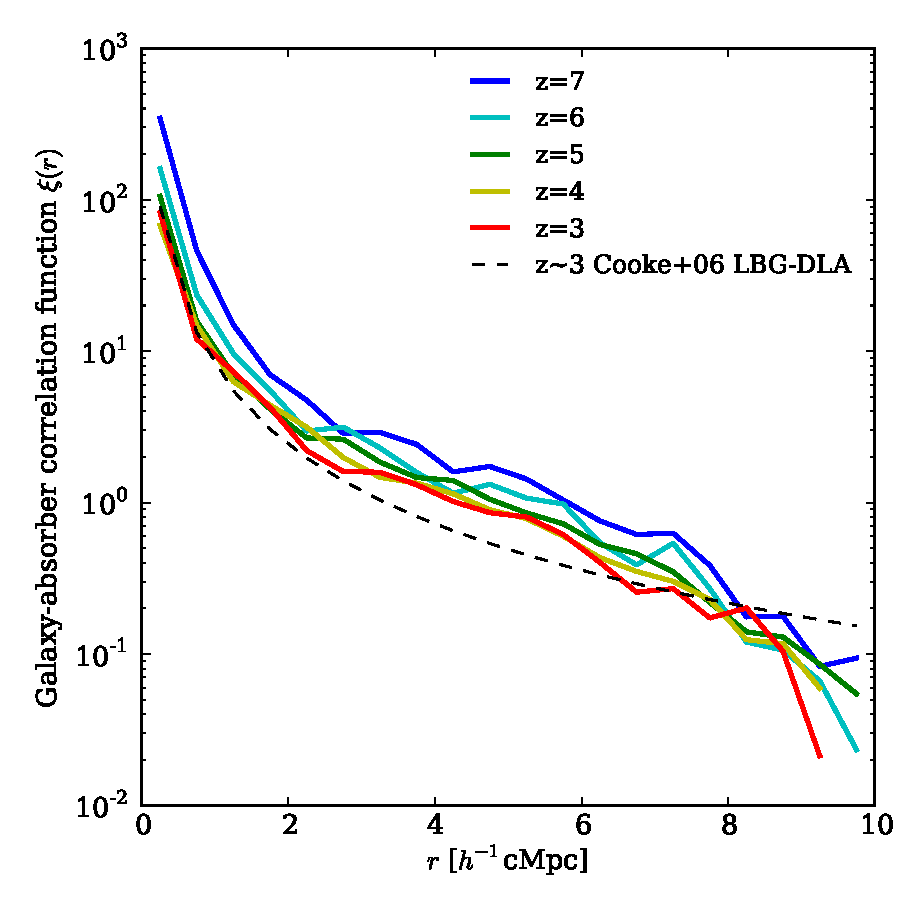
\includegraphics[angle=0,width=\columnwidth]
  {figure/2PCF_L40P256G256R0_Gamma12_SST.pdf}
  \caption{The comparision between the simulated 2PCF for different redshift 
  and the best-fit 2PCF from observation by Cooke+06.}\label{simulated_2PCF}
 \end{center}
\end{figure}

The radial component of mean pairwise velocity between galaxy and absorber
is shown in Fig.\ref{v12_z3}. We compare the linear theory, self-similar
theory, and simulations at $z=3$. As expected, the linear theory severely 
underestimate the magnitude of cosmological inflow velocity. While we allowed
the nonlinear evolution in the self-similar ansatz, which we left
the amplitude $v_in$ as a free parameter, the radial dependence has different
form when we apply the best-fit correlation function of Cooke+06.
However, the functional form derived in the self-similar ansatz provide 
a convenient functional form that can be well fitted to simulation.
The best fit parameters are $v_{in}=143$km/s, $r_{in}=8.4h^{-1}$cMpc, and
$\gamma=2.26$.

\begin{figure}
 \begin{center}
  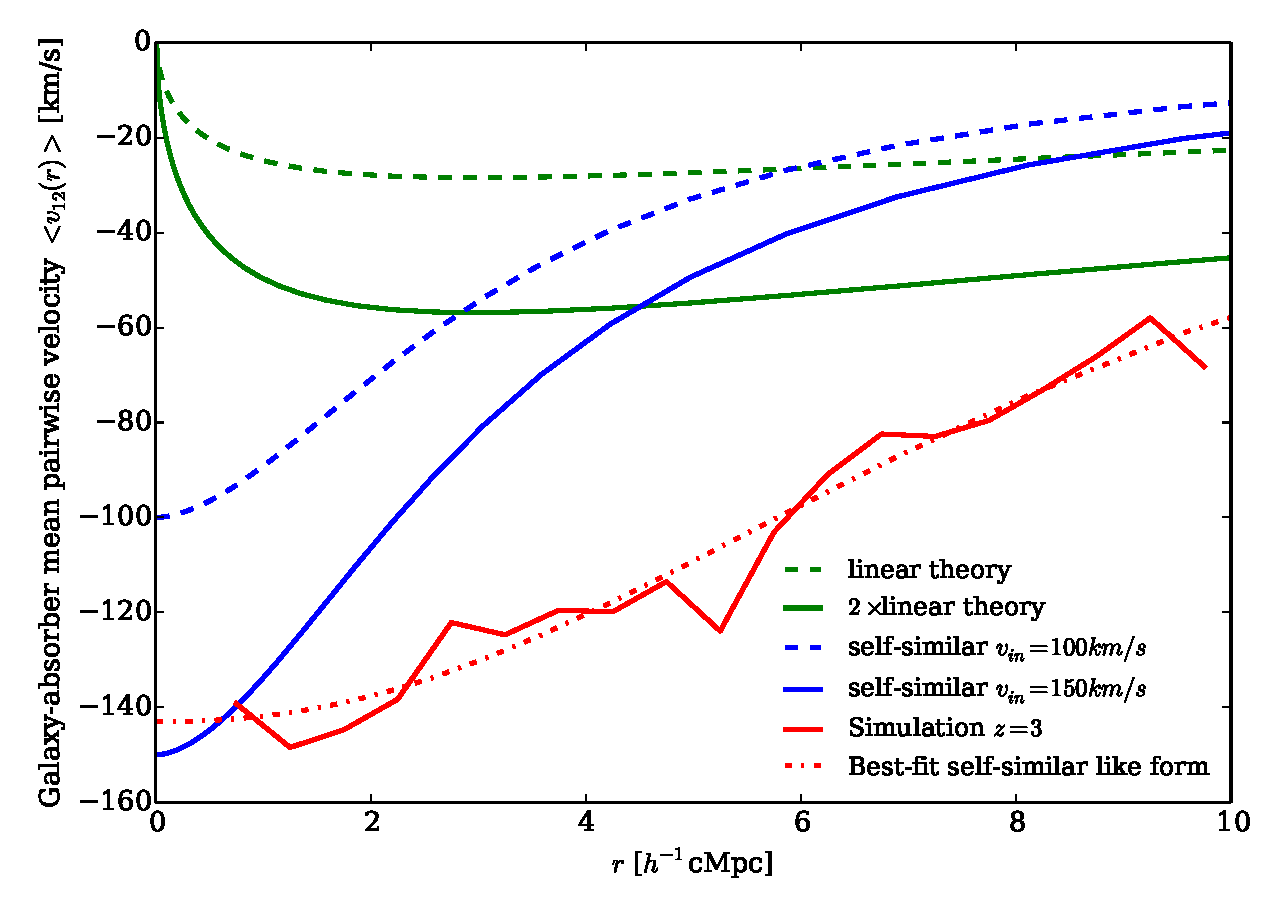
\includegraphics[angle=0,width=\columnwidth]{figure/v12_comparison_z3.pdf}
  \caption{The comparison of mean pairwise velocity between analytic theory
    and simulation at $z=3$.}\label{v12_z3}
 \end{center}
\end{figure}



\begin{figure}
 \begin{center}
  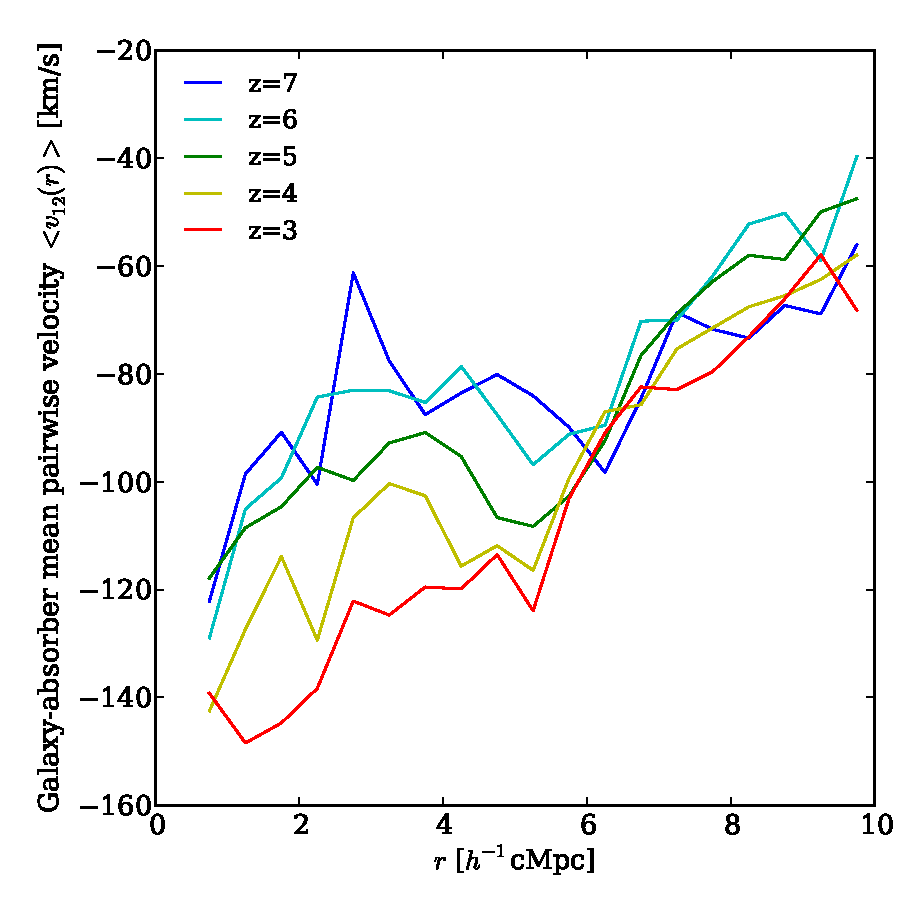
\includegraphics[angle=0,width=\columnwidth]{figure/v12_L40P256G256R0_Gamma12_SST.pdf}
  \caption{The redshift evolution of the mean pairwise velocity 
    from simulation.}\label{simulated_v12}
 \end{center}
\end{figure}




\subsection{Redshift-space distortion}


\begin{table*}
\centering
\caption{Model grids}
\label{table:model_grids}
\begin{tabular}{llllll}
\hline
&&& Available source of constraints \\
CDDF: \\
$\displaystyle\frac{\partial^2\mathcal{N}}{\partial\NHI\partial z}$ & Haardt\&Madau (2012) fit (fid.)
&& $\LyA$ forest, LLS/DLA survey\\
real-space clustering: \\
$\xi$   &  $r_0=3.32h^{-1}$cMpc (fid.)     & $\gamma=1.76$ (fid.)   &   angular correlation function\\
local photoionization effect: \\
$S$     &  $r_{eq}(f_{esc}^{LyC}SFR)=0.1,0.32({\rm{fid.}}),1.01h^{-1}$cMpc   & $\beta_N^{\rm{eff}}=2$ (fid.) 
& SFR from UV magnitude \\
&&& or SED/spectral fitting\\ 
velocity statistics: & & & primary interest of constraing by RSD\\
$v_{12}$ &  $v_{in}=100,143({\rm{fid.}}),200$km/s & $r_{in}=8.$(fid.) & $\gamma_{in}=2.26$(fid.) \\
$v_{out}=0({\rm{fid.}}),200,400,600$ & $r_{out}=1$(fid.) & & possibly helped with metal line\\
$\sigma_{12}$ &180,200(fid),220km/s  \\
\hline
\end{tabular}

\end{table*}

We consider how the RSD measurement between galaxies and absorbers helps to constrain
the pairwise velocity statistics, which is a critical ingredient to predict the 
$\LyA$ visibility affected by the intergalactic environment. While it may be 
possible to let all the model parameters free and attempt to constrain by RSD only,
we take rather a moderate approach that some model quantities can be constrained 
prior to RSD measurement. 

CDDF can be constrained by $\LyA$ forest and LLS/DLA survey. The real-space correlation
function is from the angular correlation function $\omega(\theta)$. This reduces
the parameter space to be local photoionization effect and pairwise velocity statistics.
Analysis of SED for wavelength $>1216\rm{\AA}$ can give a helpful information to characterize
the local photoionization effect such as SFR. If the metal lines are present, the outflow
velocity may be guessed.

We explore the model grids as shown in Table.\ref{table:model_grids}, which has
the total number of 13 models composed of the 3 variants of local photoionization,
and 3 variants of inflow velocity, 4 variants of outflow velocity, and 
3 variants of pairwise velocity dispersion. For each variant, the rest of paramter
is taken as the fiducial values.

\subsubsection{The variation of local photoionization}

\begin{figure*}
 \begin{center}
  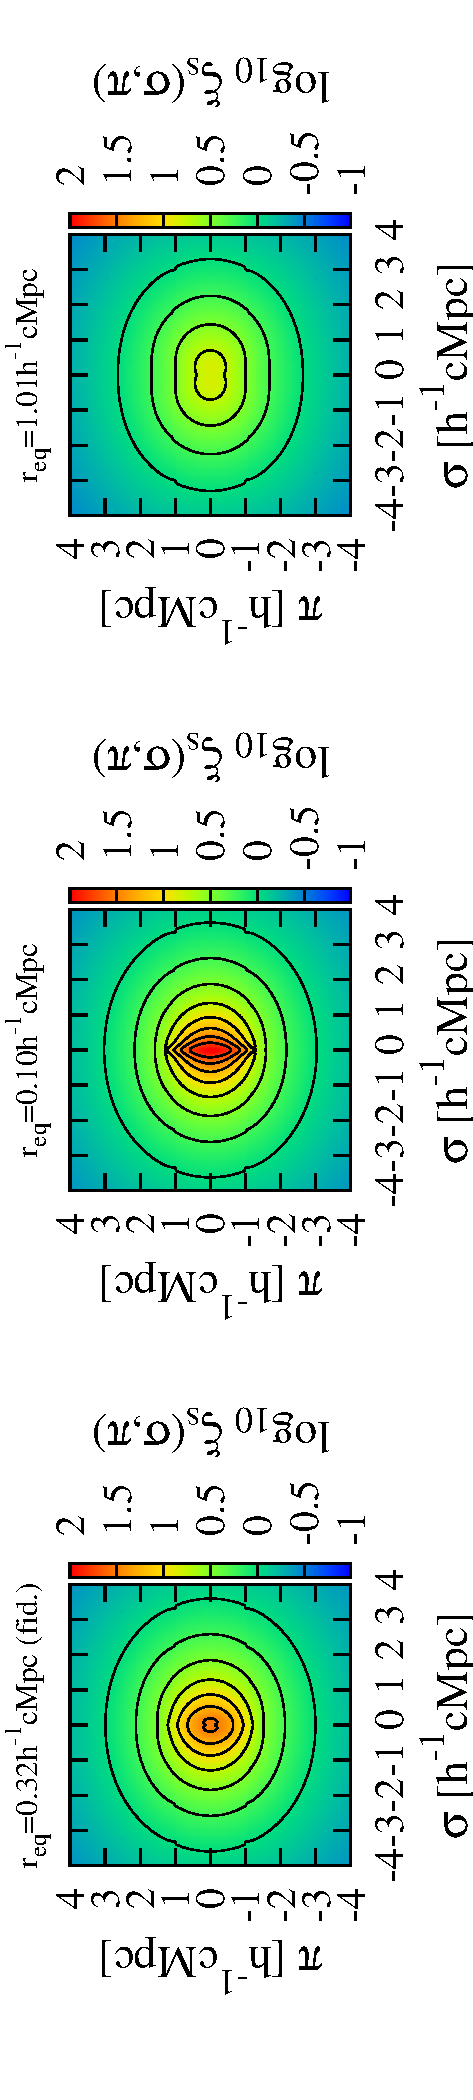
\includegraphics[angle=-90,width=\textwidth]{figure/RSDs_1-2-3.pdf}
  \caption{RSD varying the local photoionization effect.}\label{RSD_phr}
 \end{center}
\end{figure*}

\begin{figure*}
 \begin{center}
  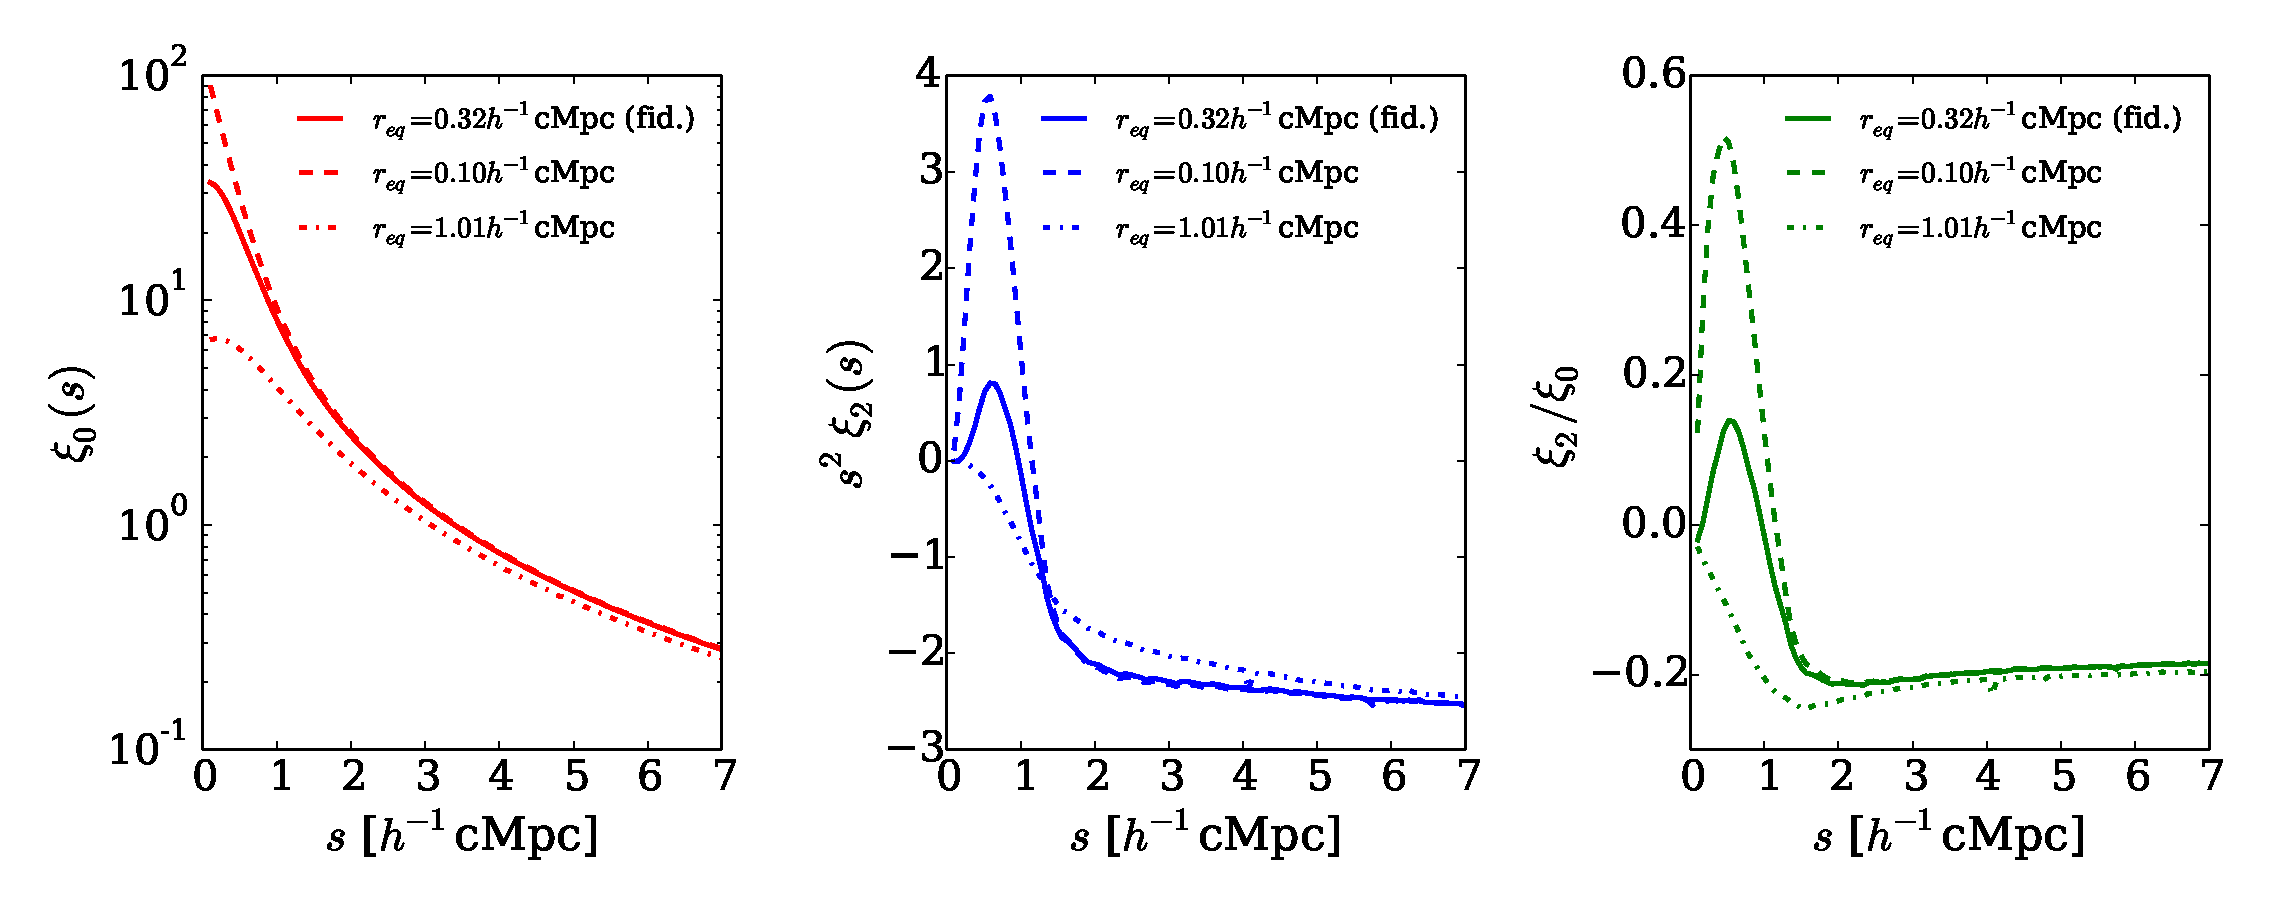
\includegraphics[angle=0,width=\textwidth]{figure/RSD_moment_model1-2-3.pdf}
  \caption{The monopole, quadrupole and monopole-quadrupole ratio of the Legendre
    moments of redshift-space correlation function.}\label{moment_phr}
 \end{center}
\end{figure*}

In Fig.\ref{RSD_phr}, we show that the 2D plot of the redshift-space correlation
function. The fiducial (left) model with $f_{esc}^{LyC}\rm{SFR}=1{\rm{M_\odot}}yr^{-1}$
is varied for low (middle) and high (right) local photoionization effect. 
The low and high photionization models correspond to 
$f_{esc}^{LyC}\rm{SFR}=0.1,10{\rm{M_\odot}}yr^{-1}$ respectively. The low
photoionization model produces the higher value of $\xi_s(\sigma,\pi)$ for 
small seperation because the real-space correlation function truncate much
smaller scale. Consequently, the figure-of-God effect on small scale become
more apparent for lower photoionization effect. More quantitative effect 
is seen in the Legendre moments of redshift-space correlation function as
shown in Fig.\ref{moment_phr}. The monopole as affected by local photoionization
effect with more small scale suppresion for higher photoionization effect.
In the quadrupole moment, this propagates as larger finger-of-God effect resulting
in the larger value of quadrupole moment for smaller scale. The monopole-quadrupole
moment is an indicator of streching (positive) and squashing (negative) of RSD.
The suppression of the small-scale power by local photoionization may
produces negative monopole-quadrupole ratio because the squashing of RSD is
weighted more in the quadrupole moment.


\subsubsection{The variation of inflow velocity}

\begin{figure*}
 \begin{center}
  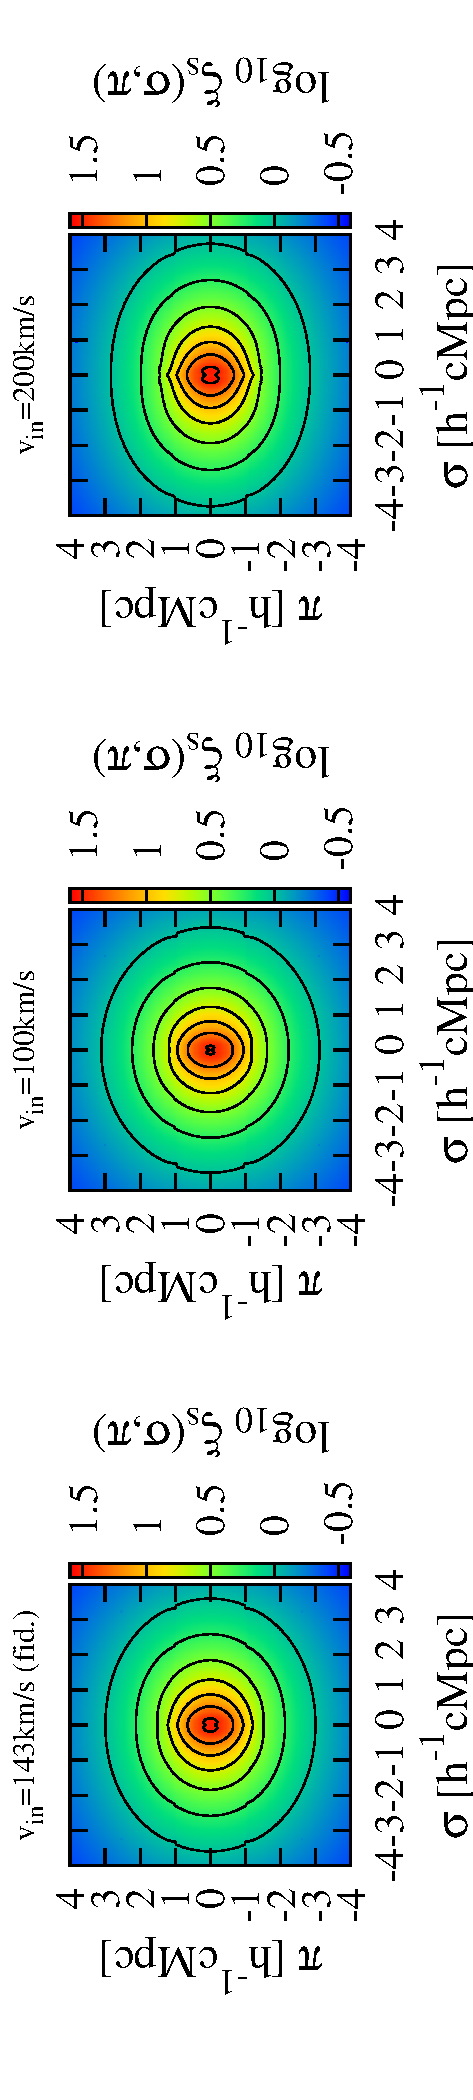
\includegraphics[angle=-90,width=\textwidth]{figure/RSDs_1-4-5.pdf}
  \caption{RSD varying the inflow velocity.}\label{RSD_inflow}
 \end{center}
\end{figure*}

\begin{figure*}
 \begin{center}
  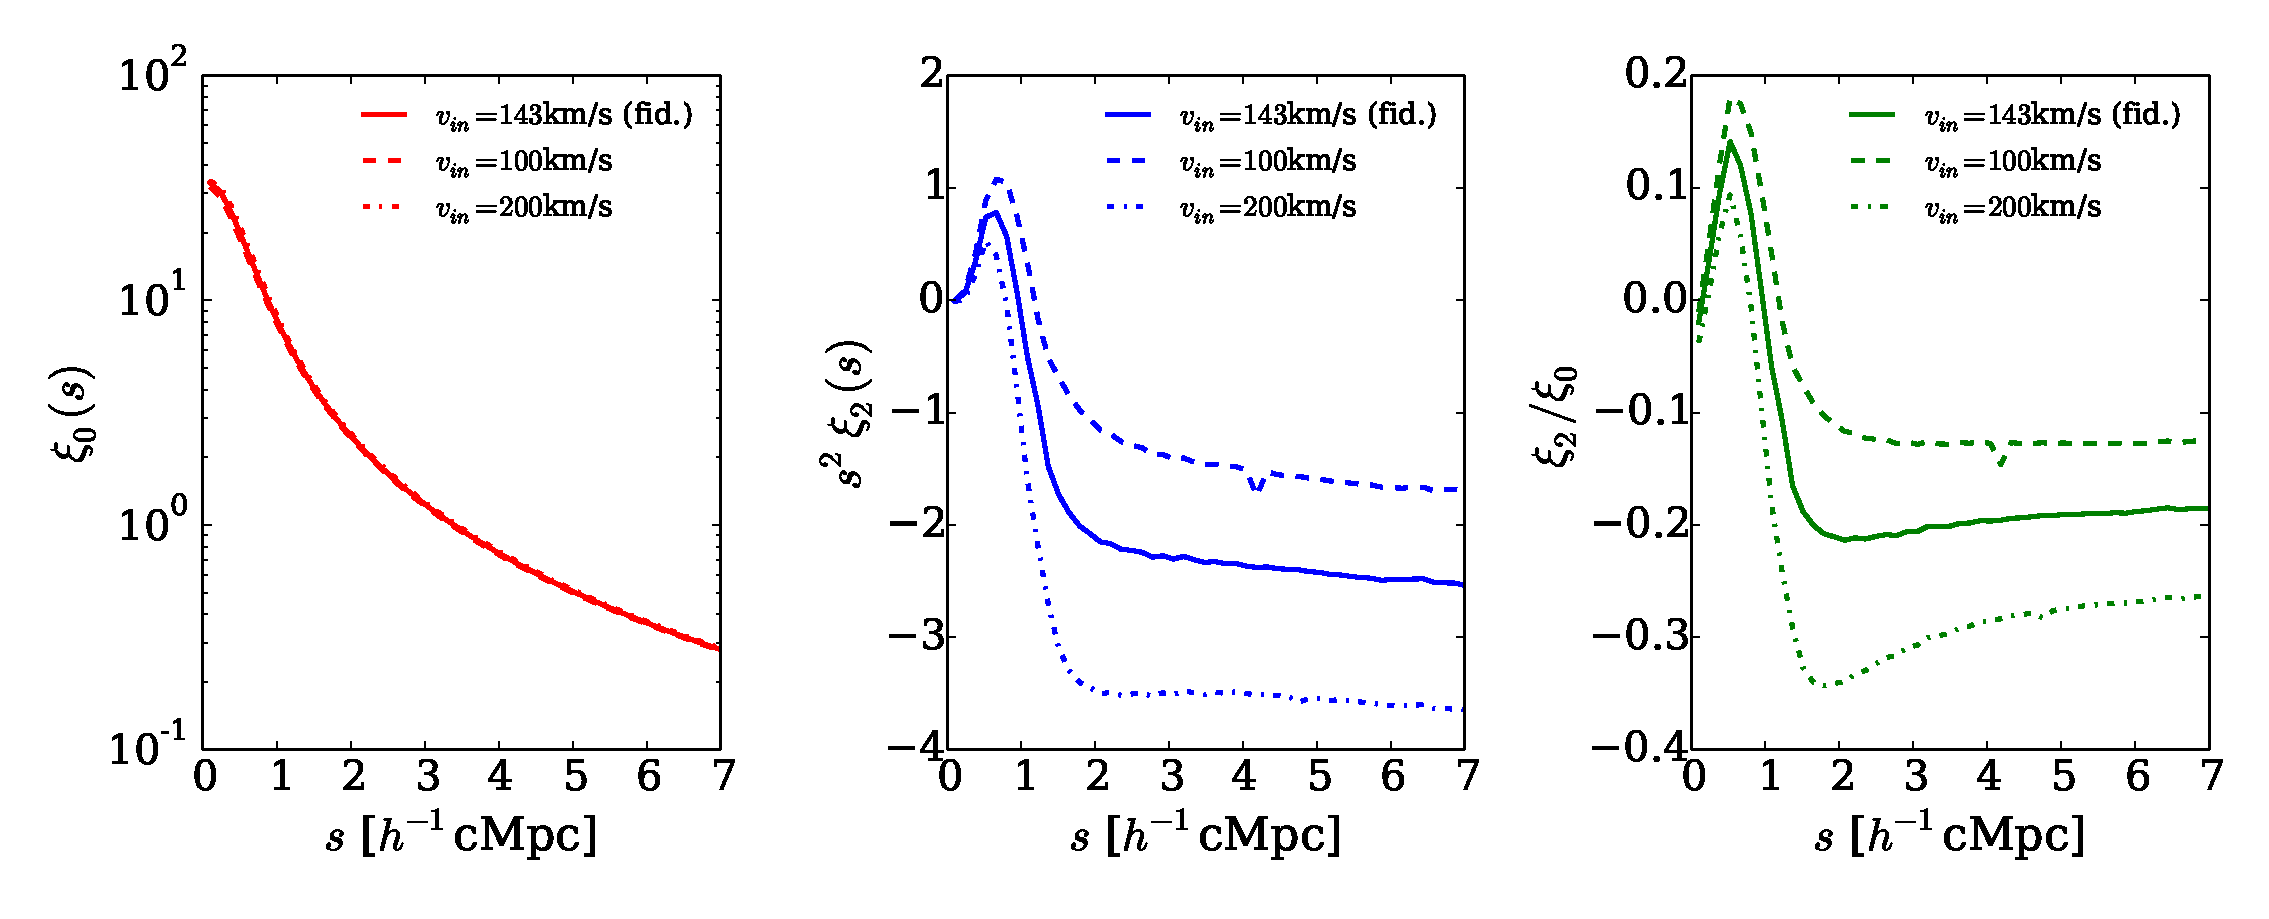
\includegraphics[angle=0,width=\textwidth]{figure/RSD_moment_model1-4-5.pdf}
  \caption{The monopole, quadrupole and monopole-quadrupole ratio of the Legendre
    moments of redshift-space correlation function.}\label{moment_inflow}
 \end{center}
\end{figure*}

Figs.\ref{RSD_inflow} and \ref{moment_inflow} show that the RSD and Legendre
moment varying the inflow velocity. As well-known (Kaiser 96?), the larger 
inflow velocity produces more squashing of the RSD. We explore how the
variation of cosmological inflow velocity affect the RSD signature.
As seen in Fig.\ref{moment_inflow}, the monopole is not affected by
the change of inflow velocity. This is understood because the change in
velocity field is washed out in the monopole moment. The quadruple and
monopole-quadrupole ratio shows the clear sign of increasing squashing of
RSD on larger scale, producing more negative value for larger inflow
velocity.


\subsubsection{The variation of pairwise velocity dispersion}

\begin{figure*}
 \begin{center}
  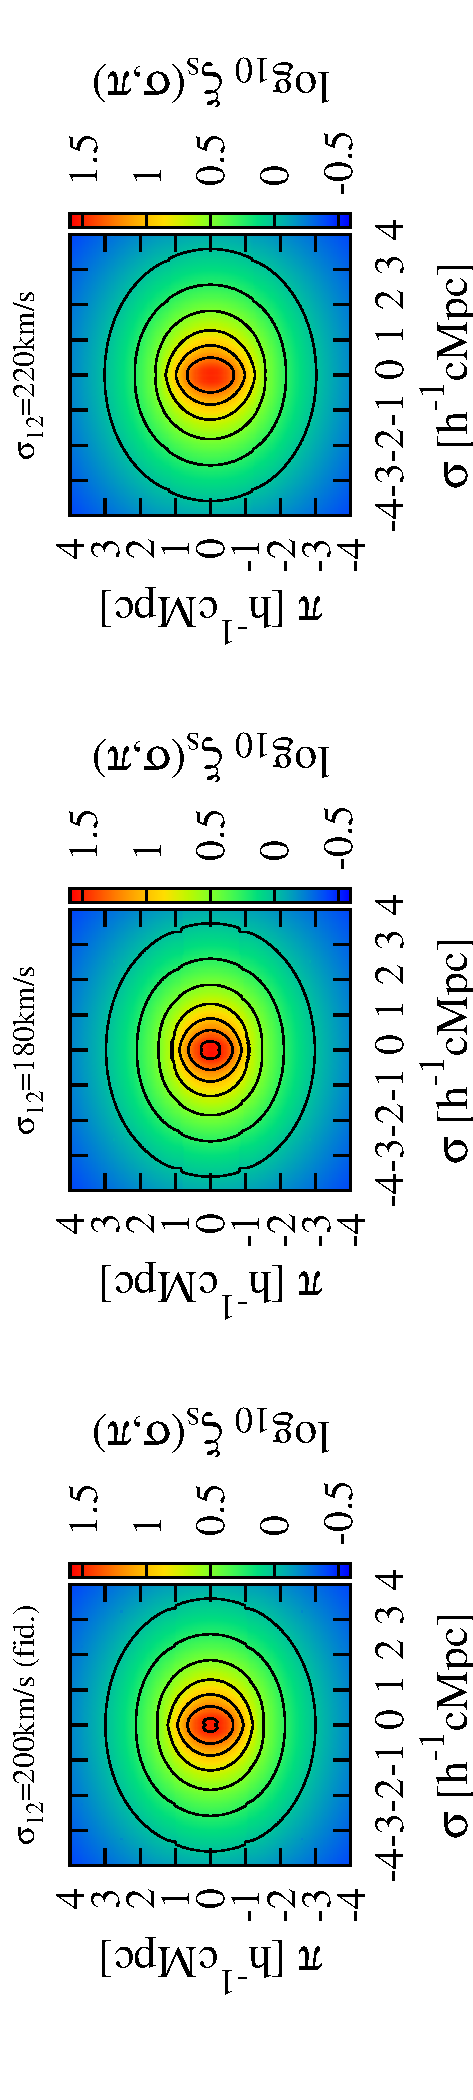
\includegraphics[angle=-90,width=\textwidth]{figure/RSDs_1-9-10.pdf}
  \caption{RSD varying the pairwise velocity dispersion.}\label{RSD_disp}
 \end{center}
\end{figure*}

\begin{figure*}
 \begin{center}
  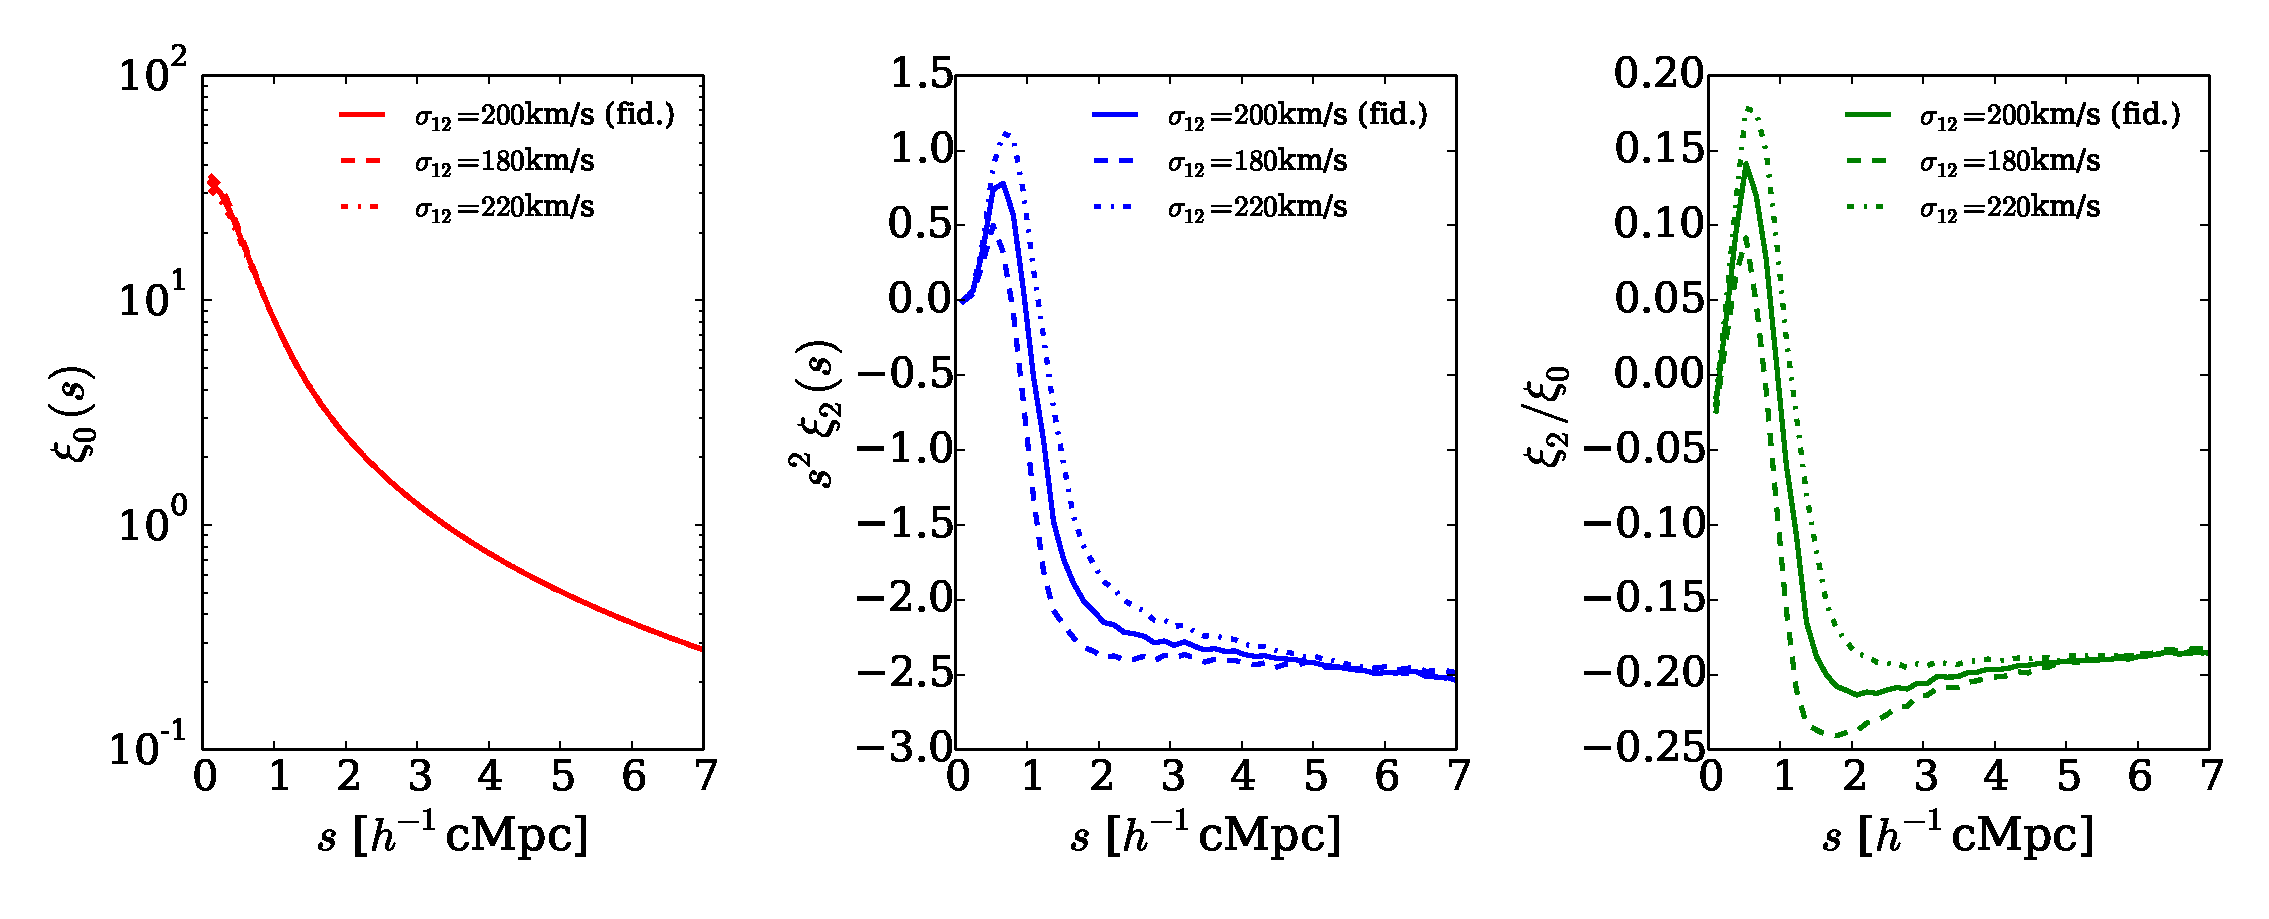
\includegraphics[angle=0,width=\textwidth]{figure/RSD_moment_model1-9-10.pdf}
  \caption{The monopole, quadrupole and monopole-quadrupole ratio of the Legendre
    moments of redshift-space correlation function.}\label{moment_disp}
 \end{center}
\end{figure*}

The variation of RSD and Legendre moments for different pairwise velocity
dispersion is shown in Figs.\ref{RSD_disp} and \ref{moment_disp}. 
Increasing Finger-of-God effect is seen for larger pairwise velocity
dispersion. Similarly to the change of inflow velocity, the monopole moment
has only a minor impact from the difference in pairwise velocity dispersion.
The amplitude of the small-scale part of the quadrupole moment varies
as a result of different size of Finger-of-God effect, while the large
scale is less affected by the pairwise velocity dispersion.


\subsubsection{The variation of outflow velocity}

\begin{figure*}
 \begin{center}
  \includegraphics[angle=-90,width=\textwidth]{figure/RSDs_1-6-7-8.pdf}
  \caption{RSD varying the outflow velocity.}\label{RSD_outflow}
 \end{center}
\end{figure*}

\begin{figure*}
 \begin{center}
  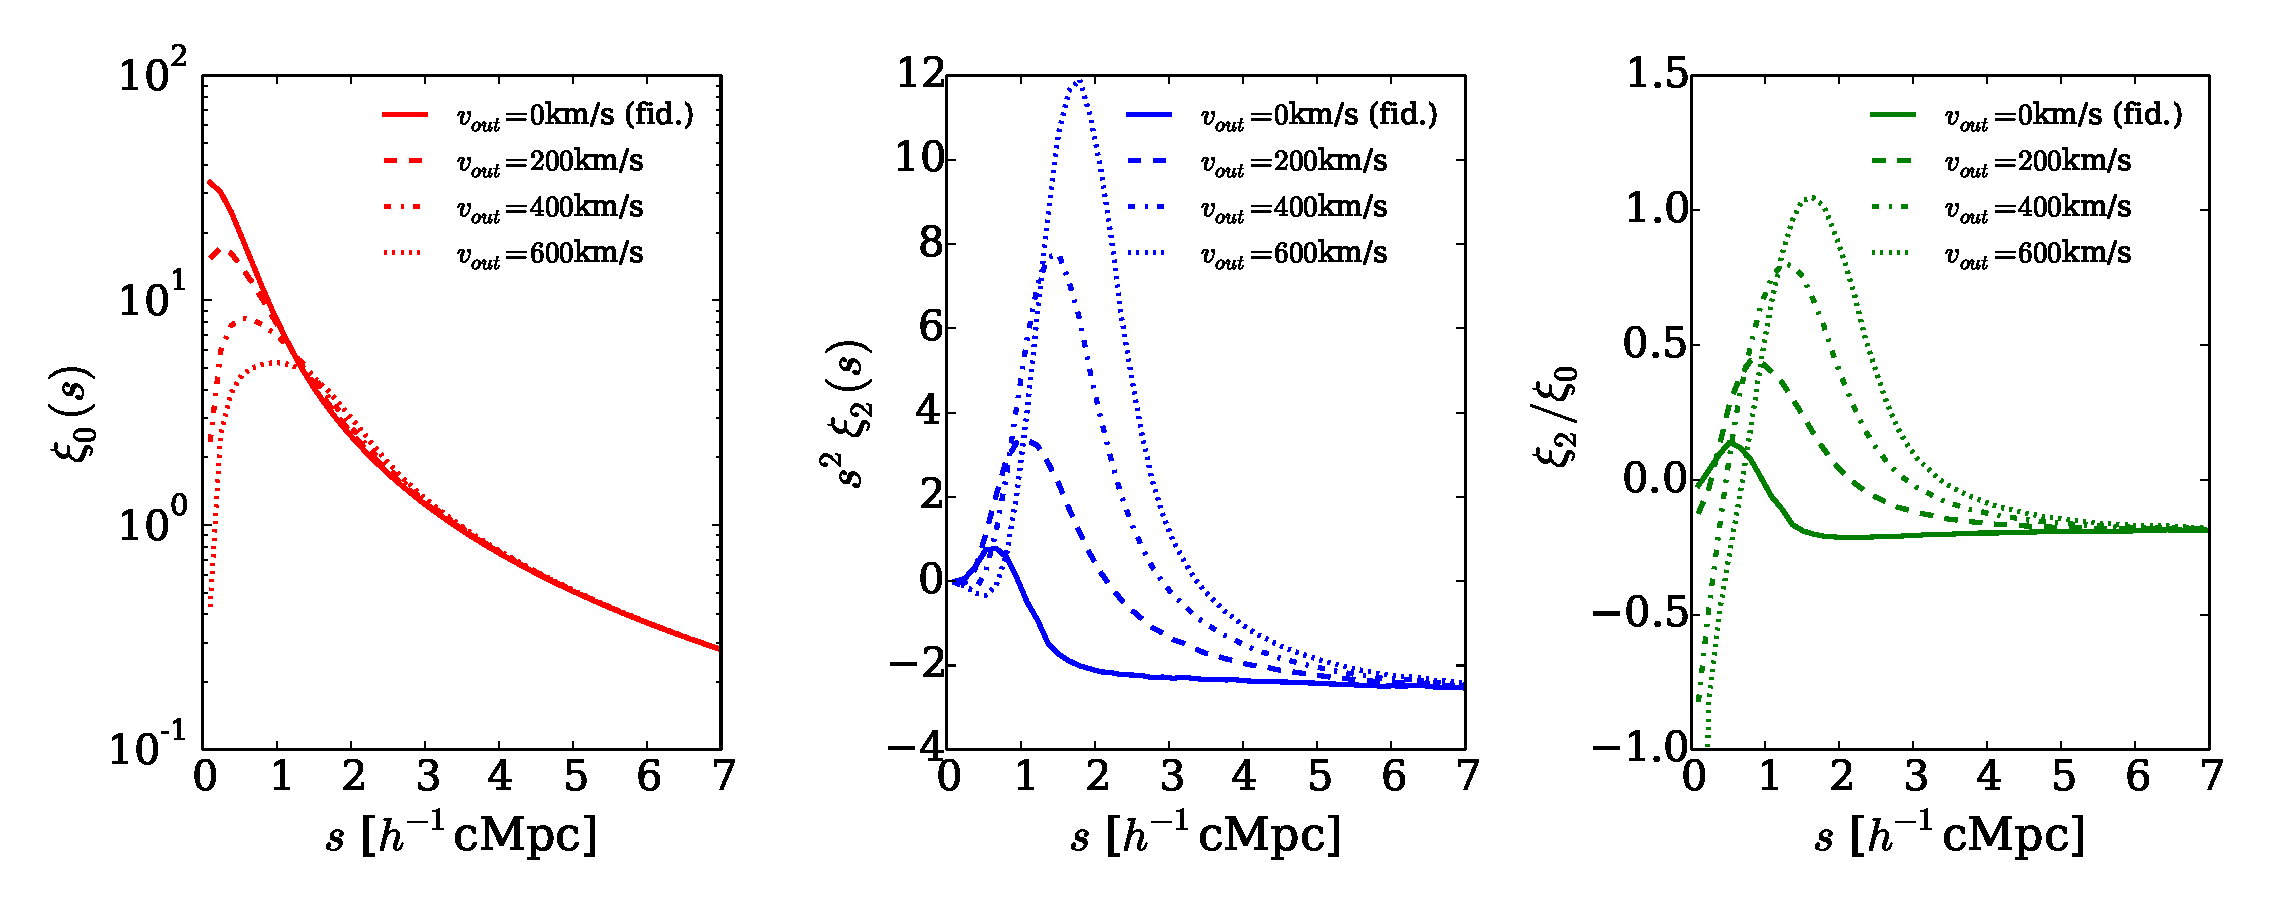
\includegraphics[angle=0,width=\textwidth]{figure/RSD_moment_model1-6-7-8.pdf}
  \caption{The monopole, quadrupole and monopole-quadrupole ratio of the Legendre
    moments of redshift-space correlation function.}\label{moment_outflow}
 \end{center}
\end{figure*}

The outflow as considered in the phenomelogical model show a peculiar signiture
in RSD as shown in Fig.\ref{RSD_outflow}. The outflow streches the RSD in the
line-of-sight direction, creating two island-like feature in the RSD.
This can be interpreted as a result of the combination of outflow and the
local photoionizaiton. Since the local photoionization creates the suppresion
of correlation function in small-scale seperation, the line-of-sight 
streching produces the islands in the RSD. The higher outflow velocity 
creates the larger line-of-sight seperation of the two islands. 

In Fig.\ref{moment_outflow}, the Legendre moments also shows the 
sign of outflow effect. Unlike the inflow and pairwise velocity dispersion,
the monopole is also affected by outflow. The apparent suppresion on
the small-scale monopole moment is the result of the line-of-sight
strech of local photoionization effect of RSD. Since the small-scale 
suppression in real-space is systematically displaced in the line-of-sight
direction, the stronger outflow produce more suppression of the monopole.
Note that since inflow displaces the local photoionization effect into
smaller scale, such effect is not visible in the monopole. Also, as the
pairwise velocity dispersion gives random displacement the effect on
monopole is very minor (but slightly larger than the impact by inflow).
The quadrupole clearly indicates the larger streching and redshift-space
displacement by outflow by pushing and amplifying the positive peak of 
quadrupole moment. Both for quadrupole and monopole-quadrupole ratio shows
that for larger scale the impact of cosmological inflow still produces 
the squashing of RSD. Finally, note that the the negative monopole-quadrupole
ratio (yet the RSD is streching) is a result of local photoionization.
Since we take the power-law slope of CDDF in the DLA regime to be 
$\beta_N^{\rm{eff}}=2$, the real-space correlation function bend to have
positive slope by strong local photoionization suppresion on smaller scale.
Hence, as the quadrupole moment positively weights in the line-of-sight
direction and negatively weights in the perpendicular direction, 
the net result is negative value of quadrupole, although the 
RSD is being streched in the line-of-sight direction.


\subsubsection{Can we handle the pairwise velocity statistics 
from RSD measurement?}

The consideration of how RSD and Legendre moments are affected by
the change in our parameters of interest to be constrained, i.e.
pairwise velocity statistics of galaxies and absorbers, helps
how well can we constrain these parameters by the RSD measurement.
As illustrated above, the local photoionization effect and the 
pairwise velocity statistics (inflow velocity, pairwise velocity
dispersion, outflow velocity) influence the RSD and Legendre
moment in different way. Fitting of RSD model provides insightful
constraints on the pairwise velocity statistics 
(\textbf{Can I do Fisher matrix forecast around a fiducial model?}).
One may hope that even in the presence of redshift error on the
galaxy and absorber position, which produces the degenrate effect to
scale-independent pairwise velocity dispersion, other interested 
parameter such as inflow velocity, may be able to constrain.


\subsection{$\LyA$ RT through the intergalactic environment}

Given the information on pairwise velocity statistics from the 
RSD measurement, we can predict the $\LyA$ opacity due to the 
intervening dynamical absorbers around galaxies.




\section{Applications}
We present a couple of interesting applications of the RSD measurement 
enabled by joint analysis of galaxy redshift survey and $\LyA$ forests
over $2<z<7$. 



\subsection{Breaking $\HI$ fraction-topology degeneracy of EoR}


\subsubsection{Strategy to break global $\HI$ fraction-topology degeneracy}
The expectation that the reionization effect on galaxy-absorber correlation
function imprinted on large-scale has very important consequence on breaking
the degenarcy between small-scale absorbers and reionization. By using small
scale RSD $r\lesssim 10h^{-1}\rm{cMpc}$ we can infer the dyanmics and
distribution of small-scale absorbers. This then inform us, as we show later,
that the effective optical $\LyA$ depth due to the small-scale absorbers
for $\LyA$-emitting galaxies. This is then compared with the observed $\LyA$
visibility $\tau=\tau_{web}+\tau_{bub}$. The required additional contribution from
$\HII$ bubble distribution inform us the global $\HI$ fraction of the IGM.
The reionization model should in turn consistently reproduce the observed 
galaxy-absorber correlation function on large-scale $r>R_b$ as a result
of $\HI$ patches outside the $\HII$ bubbles. This ability to handle the 
small-scale absorbers and reionization effect allows us to make a diagnostic
to break the global $\HI$ fraction-topology degeneracy, hence simultanously
measuring the two essential quantities of the EoR astrophysics.





\subsection{Testing $\LyA$ RT effect for HETDEX cosmology survey}
The measurement of small-scale RSD between galaxies and absorbers using
the QSO spectra allows us to test the $\LyA$ RT effect on $\LyA$-selected
galaxy cosmology survey. By masking the $\LyA$ line, we select by using
OIII line or Lyman break galaxies. Then, we measure the RSD of UV-selected
or OIII-selected (or any other ISM nebular lines) galaxies with absorbers
(this can be small sub-field of HETDEX).
Based on the statistical formalism presented above, we can predict the 
possible average $\LyA$ transmission effect. If the impact of $\LyA$ optical
depth is large, we need to take into account the $\LyA$ RT effect in clustering
measurement, whereas if the $\LyA$ optical depth is negligible it provides 
an negative evidence for $\LyA$ RT effect. However, note that RSD-$\LyA$
visibility diagnoistic does not perfectly discard the $\LyA$ RT effect since
it only takes into account the average, i.e. stacked, $\LyA$ visibility.
If the substaintial spatial variation of IGM environment of $\LyA$-emitting
galaxies is possible, only charactering the mean visiblity is not sufficient
to argue that $\LyA$ RT effect is negible in HETDEX. This case the repeating
RSD diagnostic for different sub-fields would give an insight on the 
variation of IGM environment of $\LyA$-emitting galaxies. 





\section{Survey Requirements}
We propose the sketch of survey requirement to characterise the IGM/CGM 
environment of $\LyA$-galaxies for $2<z<7$.

\subsection{QSO fields}
\begin{table}
\centering
\caption{List of potential targets of QSO fields. QSOs used in Fan+2006 and 
Becker+2014 are listed. Also three QSOs from Pan-STARRS1 survey (Venemans+15).} \label{table:qso_field}
\begin{tabular}{lll}
\hline
QSO name                               & QSO redshift  &         \\ 

\hline
$z>6$            &      \\
PSO J338.2298+29.5089             &  6.658        & Venemans+15 \\
PSO J036.5078+03.0498             &  6.527        & Venemans+15 \\
PSO J167.6415-13.4960             &  6.508        & Venemans+15 \\
SDSS J1148+5251                   &  6.4189       & Fan+06  \\
SDSS J1030+0524                   &  6.3110       & Fan+06  \\
CFHQS J0050+3445                  & 6.25 \\
SDSS J1623+3112                   &  6.2470       & Fan+06  \\
SDSS J1048+4637                   &  6.2284       & Fan+06  \\
SDSS J125051.93+313021.9          &  6.1300       & Fan+06  \\
ULAS J1319+0950                   & 6.13 \\
SDSS J2315−0023                   & 6.12 \\
SDSS J1602+4228                   &  6.0700       & Fan+06  \\
SDSS J1630+4012                   &  6.0650       & Fan+06  \\
SDSS J2054−0005                   & 6.06 \\
SDSS J0353+0104                   & 6.05 \\
SDSS J0818+1722                   & 6.02         & Fan+06  \\
SDSS J1306+0356                   &  6.0160       & Fan+06  \\
SDSS J113717.73+354956.9          &  6.0100       & Fan+06  \\
\\
$5<z<6$ \\
ULAS J0148+0600                   & 5.98 \\
SDSS J1411+1217                   &  5.9270       & Fan+06  \\
SDSS J133550.80+353315.8          &  5.9012       & Fan+06  \\
SDSS J0005-0006                   &  5.85         & Fan+06  \\    
SDSS J0840+5624                   &  5.8441       & Fan+06  \\
SDSS J143611.74+500706.9          &  5.8300       & Fan+06  \\
SDSS J104433.04-012502.2          &  5.7824       & Fan+06  \\
SDSS J0836+0054                   &  5.774        & Fan+06  \\
SDSS J092721.82+200123.7          &  5.7722       & Fan+06  \\
SDSS J0203+0012  & 5.72 \\
SDSS J0231−0728  & 5.42 \\ 
SDSS J1659+2709  & 5.32 \\
SDSS J1208+0010  & 5.27 \\
SDSS J0915+4244  & 5.20 \\
SDSS J1204−0021  & 5.09 \\
\\
$4<z<5$ \\
SDSS J0040−0915  & 4.98\\
SDSS J0011+1446  & 4.95\\
SDSS J2225−0014  & 4.89\\
SDSS J1616+0501  & 4.88\\
BR 1202−0725     & 4.70\\
SDSS J2147−0838  & 4.60\\
BR 0353−3820     & 4.59\\
BR 1033−0327     & 4.52\\
BR 0006−6208     & 4.52\\
BR 0714−6449     & 4.49\\
BR 0418−5723     & 4.48\\
\\
$z<3-4$ \\
see BOSS $\LyA$ survey & & Kee-Gee?+ \\
  \hline
\end{tabular}

\end{table}

Firstly, the selection of the potential target fields is listed in
Table $\ref{table:qso_field}$. The redshift range covered by the $\LyA$ 
forest between $\LyA$ and $\mbox{Ly}\beta$ lines in the restframe of a 
background QSO at redshift $z_Q$ is $\Delta z/(1+z_Q)=\Delta\lambda/
\lambda_\alpha$ where $\Delta\lambda=\lambda_\alpha-\lambda_\beta$ is the 
wavelength interval between $\LyA$ and $\mbox{Ly}\beta$ lines.

To perform the Voigt profile decomposition of $\LyA$ forests, both high 
signal-to-noise ratio per pixel and high resolution ($\rm{FWHM\lesssim25km/s}$)
spectroscopy of a QSO should be obtained (\citealt{1998ARA&A..36..267R}). 
For example, KBSS survey (\citealt{2012ApJ...750...67R}) has observed 
15 QSOs with Keck/HIRES, obtaining $R\simeq45000$ 
(FWHM$\simeq 7$km/s) and $\rm{S/N\sim50-200pixel^{-1}}$. The resolved FWHM sets 
the lower limit of $b$-parameter can be measured from voigt profile 
decomposition. 

While the high resolution and high S/N spectroscopy is always desirable 
whenever available, there are a couple of ways to characterise the absorbing 
systems with the equivalent width and redshift using intermediate resolution 
spectroscopy (\citealt{1998ARA&A..36..267R}). We explore the pixel optical 
depth method, EW-redshift indentification, and voigt profile decomposition 
to characterise the CGM/IGM environment using the synthetic spectra from 
simulations in the subsequent section. 


\subsection{Galaxy fields}
\begin{table*}
\centering
\caption{Telescopes and intruments for redshift surveys with $\LyA$ forests}
\label{table:telescope}
\begin{tabular}{llll}
\hline
Telescope/Instrument & Field of View          & Pixel resolution   & Ref. \\
                     & [arcmin$\times$arcmin] & [arcsec/pixel]     &  \\
\hline
\underline{Imaging} \\
Subaru/Supreme-Cam & $34'\times27'$           & 0.202              & Ouchi+2008 ++ \\
HST/WFC3(ACS)      & $ \sim2.1' ()$           & 0.128              & Ellis+2012 (HUDF12)  \\
Magellan/IMACS     & $27.2'\times27.2'$       & 0.2                & Dressler+2014 \\ 
\hline
\underline{Spectroscopy} \\
Keck/HIRES \\
Keck/DEIMOS \\
VLT/X-Shooter \\
Gemini/GMOS \\
\hline
\end{tabular}

\end{table*}

\begin{table*}
\centering
\caption{Future telescopes and intruments for redshift surveys with $\LyA$ forests}
\label{table:telescope}
\begin{tabular}{llll}
\hline
Telescope/Instrument & Field of View          & Pixel resolution   & Ref. \\
                     & [arcmin$\times$arcmin] & [arcsec/pixel]     &  \\
\hline
\underline{Imaging} \\
Subaru/HSC &            &              &  \\
ELT &            &              &  \\
JWST &            &              &  \\
\hline
\underline{Spectroscopy} \\
Subaru/PFS \\
\hline
\end{tabular}

\end{table*}


\subsubsection{Angular coverage}
The angular coverage of a survey should be large enough that the region
$\LyA$ RT influence is well included. $\theta_{\rm{infl}}=D_{\rm{infl}}/D_A(z)$
where $D_A$ is the angular diameter distance. This requirement is easily
met for most of telescope with a single field-of-view (FoV), e.g.
for Subaru/Supreme-Cam $34'\times27'$ FoV.

The region of influence can extend as large as $\sim50h^{-1}\rm{cMpc}$ for
DLAs, whereas it is as small as $\sim2h^{-1}\rm{cMpc}$ for LLS. Since the 
angular size of the region of influence (ca. 10-100arcmin) stays approximately 
constant, the same mosaicing can be applied to survey the wide range of redshift.
For the Subaru/Magellan-like ground-based telescope, the region of influence of
LLSs can be covered by the single field of view. For DLA, the several mosaicing,
say 2-7 tiles for one direction, is required. For the HST-like space-based telescope, 
also for JWST, order of 10 tiles for LLS and of 100 tiles for DLA are required.

Note that the estimate of the region of influence presented here only includes 
the Hubble flow. The systematic deviation due to peculiar velocity by the large-scale
structure formation produces inflow. In the presence of large-scale inflow,
the comoving region of influence will become larger.
 
\begin{figure}
 \begin{center}
  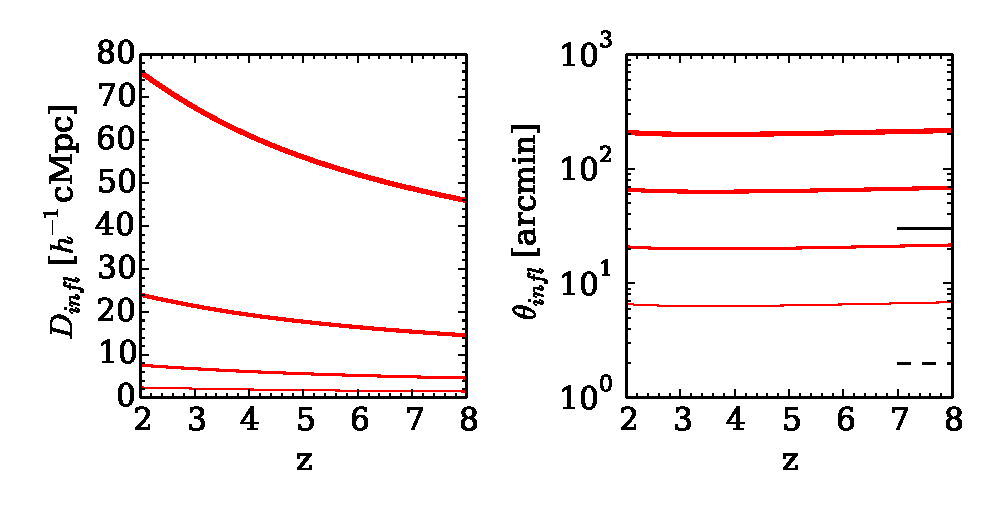
\includegraphics[angle=0,width=\columnwidth]{figure/region_of_influence.pdf}
  \caption{The comoving region of influence (left pannel) and the angular size on the sky 
  (right pannel) for the strong absorbers with column density 
  $\NHI=10^{19},10^{20},10^{21},10^{22}\rm{cm}^2$
  (from bottom to top). The field-of-views of the Subaru/Magellan-like ground-based 
  telescope (30arcmin, solid) and HST-like space-based telescope (2arcmin, dashed) 
  are shown as horizontal black lines.}
 \end{center}
\end{figure}

\subsubsection{Spectroscopic requirement}
The redshift error of objects ($\LyA$ forests and galaxies) should
be below the inflow or outflow velocity scale that we want to probe.
For $z=2-3$ LBGs, \cite{2010ApJ...717..289S} observed using metal lines that the large-scale
galactic outflow spans over 100km/s-600km/s. To gain the velocity space error
below 100km/s, the required absolute redshift error should be below 
$\Delta z=\delta v/c=0.0003$. In terms of spectroscopy, the spectral
resolution should exceed $R=\lambda/\Delta\lambda=(1+z)/\Delta z\approx
3000(1+z)$.


\subsubsection{Number counts of LAE/LBG selections}

We estimate the expected number counts of $\LyA$/UV-selected galaxies 
in the QSO field within the field-of-view to cover the region of influence.
The required flux limit provide the feasiblity of such survey strategy. 

The expected number of galaxies within the survey volume is
\begin{equation}
N(>F_{lim})=\Omega_{survey}\int_{z_1}^{z_2} dz\frac{d^2V}{dzd\Omega}\int_{4\pi D_L^2(z)F_{lim}}^\infty
\frac{dn(>L,z)}{dL}dL
\end{equation}
where $\frac{d^2V}{dzd\Omega}=\left|\frac{dr}{dz}\right|D_A^2(z)$ and
we have assume plane-parallel approximation and $\bar{z}$ is the mean
redshift depth of the survey. $z_1=z_Q-\Delta z$ and $z_2=z_Q$. Since the obseravtion
showed that for $z=3-6$ the LAE luminosity function evolves very slowly,
for Schecter fit $\phi(L)dL=\phi_\ast(L/L_\ast)^{\alpha}e^{-L/L_\ast}dL/L_\ast$,
\begin{equation}
N(>F_{lim})\approx\Omega_{survey}
\int_{z_1}^{z_2}\frac{cD_A^2(z)dz}{H(z)}
\phi_\ast \Gamma\left(1+\alpha,\frac{4\pi D_L^2(z)F_{lim}}{L_\ast}\right)
\end{equation}
where $\Gamma(a,x)$ is the upper incomplete Gamma function.


\begin{figure}
 \begin{center}
  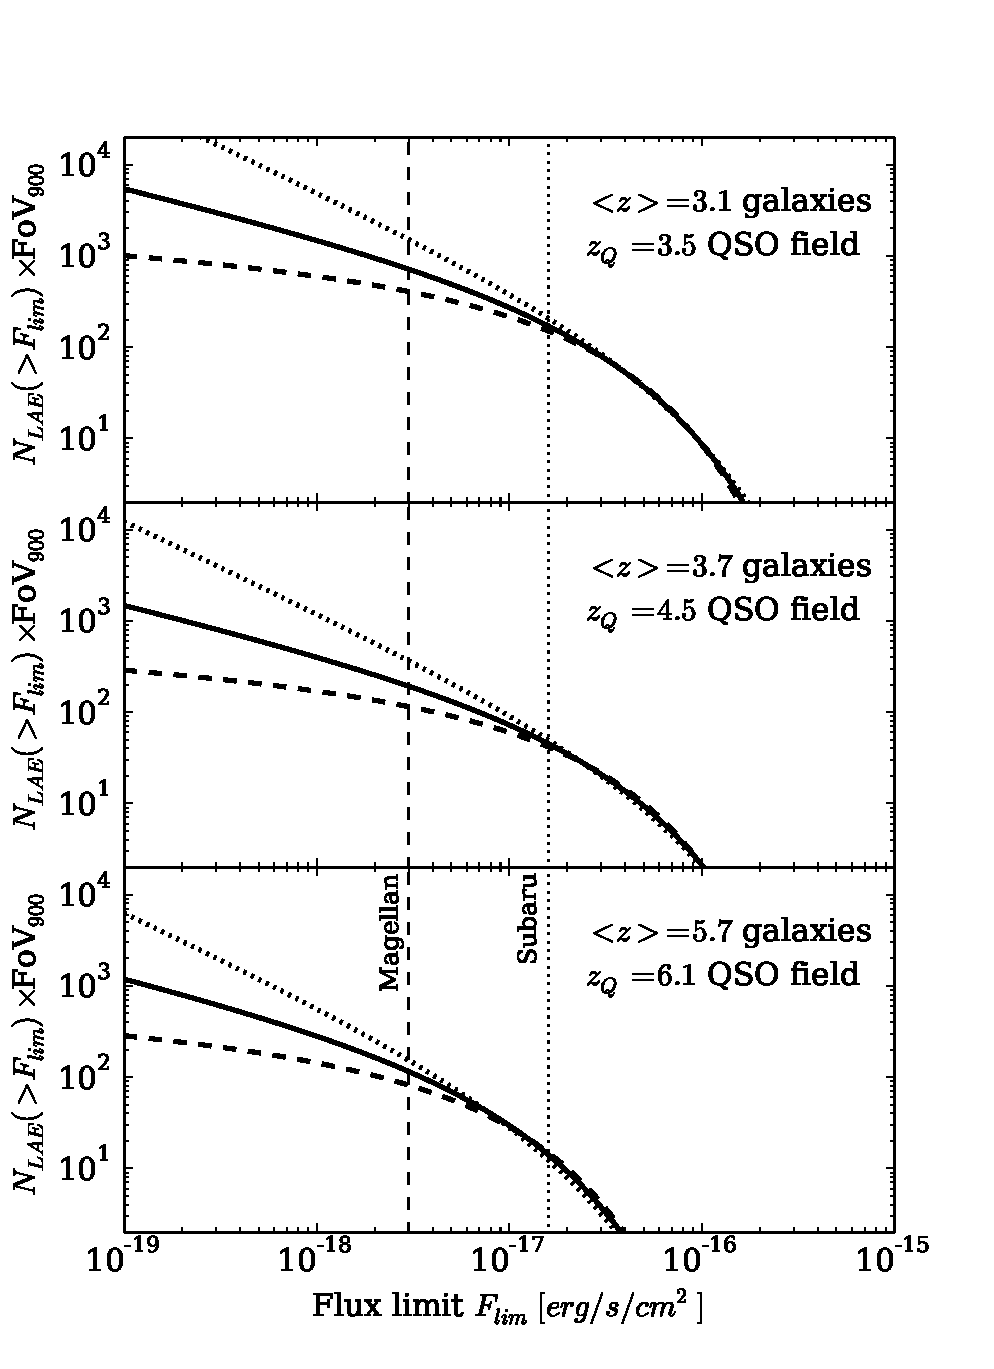
\includegraphics[angle=0,width=\columnwidth]{figure/LAE_number_counts.pdf}
  \caption{The expected number counts of LAEs in redshift galaxy survey in candidate QSO fields
    for $3<z<7$. y-axis shows the LAE number counts in a $30\times30$arcmin$^2$ field-of-view 
    $\rm{FoV_{900}=(FoV/900arcmin^2)}$. The vertical lines show the practical flux limit for
    current survey using Subaru/Supreme-Cam (dotted; Ouchi+2008) and Magellan/IMACS 
    (dashed; Dressler+2014). The LAE luminosity function is taken from the best-fit Schecter
    function of Ouchi+(2008) with three fixed faint-end slope, $\alpha=-1.0, 1.5, 2.0$ (dashed,
    solid, dotted lines). We assumed the entire $\LyA$ forest region between 
     $\LyA$ and $\mbox{Ly}\beta$ lines is covered by the survey. }
 \end{center}
\end{figure}

\begin{figure}
 \begin{center}
  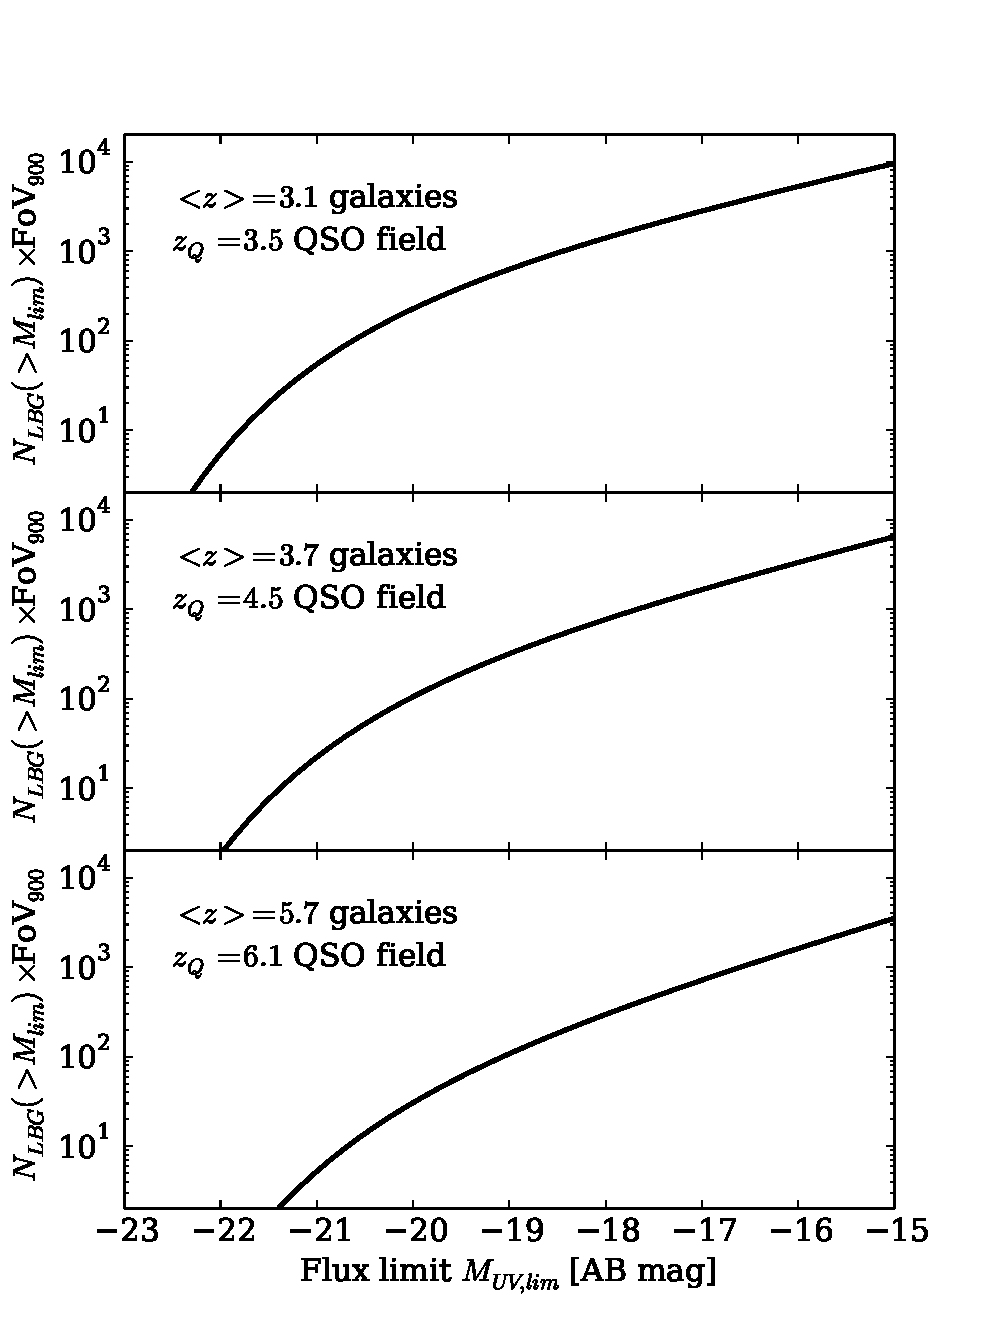
\includegraphics[angle=0,width=\columnwidth]{figure/LBG_number_counts.pdf}
  \caption{The expected number counts of LBGs in redshift galaxy survey in candidate QSO fields
    for $3<z<7$. y-axis shows the LBG number counts in a $30\times30$arcmin$^2$ field-of-view 
    $\rm{FoV_{900}=(FoV/900arcmin^2)}$. The LBG UV luminosity function is taken from the best-fit 
    Schecter function of Bouwens+(2014). We assumed the entire $\LyA$ forest region between 
     $\LyA$ and $\mbox{Ly}\beta$ lines is covered by the survey. }
 \end{center}
\end{figure}

\subsubsection{Galaxy-absorber pair counts}


\begin{figure}
 \begin{center}
  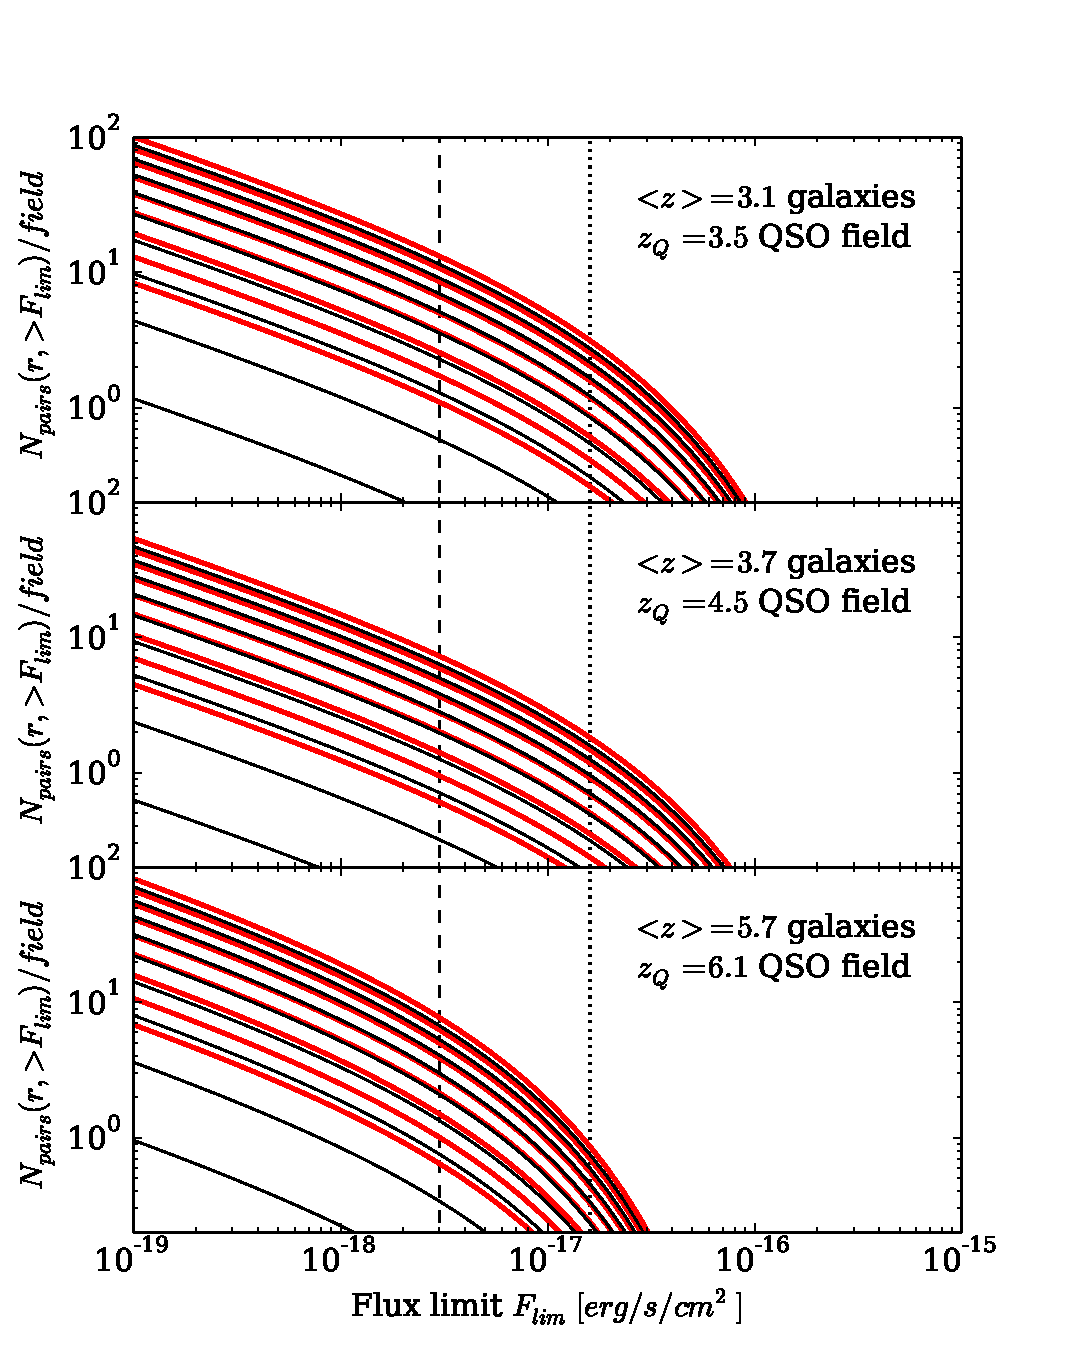
\includegraphics[angle=0,width=\columnwidth]{figure/LAE_pair_counts.pdf}
  \caption{The expected number of LAE-absorber($\NHI>10^{19}cm^{-2}$) pairs per
QSO field as a function of flux limit. The red lines are the case with 
galaxy-absorber clustering and black lines are for no clustering. 
The pair for each radial bins are 10,9,8,7,6,5,4,3,2,1$h^{-1}$cMpc
with bin size of $1h^{-1}$cMpc from top to bottom. The vertical lines
are Magellan/IMACS like instrument (dashed) and Subaru/Supreme-Cam like 
instrument (dotted).}\label{LAE_pair_counts}
 \end{center}
\end{figure}

To measure the galaxy-absorber correlation function, we need to sample
the sufficient number of the galaxy-absorber pairs to lower the random
sampling error. For the simple case of Poisson error estimate, the random 
uncertainty in the correlation function is $\frac{\Delta \xi(r)}{1+\xi(r)}
=1/\sqrt{N_{pair}(r)}$, which is the lower bound of more realistic error 
(Peacock 1998). To measure the correlation function below $10\%$ error,
more than 100 pairs per bin are required. The expected number of galaxies 
centred at each absorber ($N_{a,pair}(r)=N_{pair}(r)/\mathcal{N}$) is 
$N_{a,pair}(r)=\frac{4\pi R^3}{3}\int_{L_{lim}}^\infty\frac{dn}{dL}
\int_{r-\frac{1}{2}\Delta r}^{r+\frac{1}{2}\Delta r}p(r)dr$ where $R$ is the radius
of survey field-of-view and $p(r)dr$ is the 
probability that a galaxy is found in the interval $r$ and $r+dr$ around an 
absorber. For the Poisson distribution of galaxies, 
$p(r)dr=4\pi r^2dr/((4\pi/3)R^3)$. If one expects some degree of clustering
around an absorber, the probability is modifed as 
$p(r)dr=4\pi r^2[1+\xi^{expt}(r)] dr/[(4\pi/3)R^3]$ where $\xi^{expt}_{ag}(r)$ 
is the expected absorber-galaxy correlation function.
Thus, the total number of galaxy-absorber pairs for each bin $\Delta r$ for
each QSO field is given by $N_{pair}(r)=\mathcal{N}N_{a,pair}$,
\begin{equation}
N_{pair}(r)=\mathcal{N}\int_{L_{lim}}^\infty\frac{dn}{dL}dL
\int_{r-\frac{1}{2}\Delta r}^{r+\frac{1}{2}\Delta r}
4\pi r^2\left(1+\xi^{expt}_{ag}(r)\right)dr.
\end{equation}
The linear theory expectation of galaxy-absorber correlation function is 
$\xi_{ag}^{lin}(r)=b_ab_g\int \Delta^2(k)\frac{\sin kr}{kr}dk (check!)$
where $b_a$ and $b_g$ are the linear bias of absorbers and galaxies 
respectively. For $2<z<3$ BOSS, $b_{LyF}$, $b_{DLA}$. $b_{LAE}$ $b_{LBG}$. 
The expected number of absorbers for each QSO spectrum is
\begin{equation}
\mathcal{N}(\NHI)=\int_{z_1}^{z_2}dz\int_{\NHI^{min}}^{\NHI^{max}}d\NHI 
\frac{d^2\mathcal{N}}{d\NHI dz}
\end{equation}

Fig.$\ref{LAE_pair_counts}$ shows that expected galaxy-absorber pair
counts. We have assumed the fixed power-law correlaction function
$\xi(r)=(r/r_0)^{-1.74}$ (Cooke+2003) and the CDDF (O'Meara+2012).

\subsection{Survey strategy}
Fig.$\ref{LAE_pair_counts}$ guides us the first estimate of the survey
strategy to measure the correlation function between galaxy and absorber.
If we employ the present Magellan/IMACS like intrument, it is feasible
to measure the correlation function with $\sim10-30\%$ Poisson error by
observing the multiple QSO fields (ca. $\sim 10$ QSO fields) as we expect
to see $10-100$ pairs per radial bin.
The single deep QSO field of futuristic flux limit $10^{19}erg/s/cm^2$
can give the similar Poisson error.

In the following treatment, we construct the mock survey to study the 
survey strategy and the feasiblity in more detail.



\section{Discussions}

\subsection{Case for saturating $\LyA$ forests}
use Ly-beta forest. or extrapolate low-z to high-z. note that
from $z\sim5$ to $z=7$ only 400Myr time interval.

One approach is to employ the cosmological hydrodynamical simulations
calibrated to match the RSD measurement of galaxy-absorber correlation function.
Suppose the simulations are calibrated against $z=2-4$ measurements. Then,
the expected evolution of galaxy-absorber phase space dynamics to higher 
redshift $z>6$ allow us to perform the simulation-aided measurement of
global $\HI$ fraction with breaking the degeneracy with reionization topology.


\subsection{Low-ionization metal (ISM) lines}
The absorption lines of the low-ionization metals (CIV? etc) is detected
for $z=2-3$ galaxies, typically blueward of line centre as interpreted
as metal-enriched outflow. 
ISM lines suppliments the modelling of the intrinsic $\LyA$ line. 
Self-consistent modelling of both ISM lines and $\LyA$ line would confine
the parameter space for outflow of model galaxies. Hence it offers a 
possibility to break the intrinsic galaxy property - IGM environment 
degenracy on $\LyA$ visibility. If correlation with UV magnitude with
$\LyA$ line profile (esp. line shift) the calibration of model with
ISM line-detected galaxies would help to peeling into EoR era and
more robust measurement of IGM neutral fraction.
 


\subsection{Synergy with 21cm radio interferometry}
While we have restricted ourselve in near-infrared observation with telescope
such as HST, Subaru, Keck, VLT. When the radio interferometric observations
become available, the combined analysis offer a way to explore deeper into
the EoR. One possible way is to utilize 21cm forests, which unlike 
$\LyA$ forests provides the unsaturated spectrum encoding the small-scale
IGM structures. Hence the absorber-galaxy redshift-space distortion may be
measured by galaxies and 21cm forests. Of course, the availability of number
of 21cm forest sightlines is still questionable due to the lack of high-redshift
radio-loud objects. Nonetheless, it is worthwhile to keep our mind open 
for this oppotunity.  

 


%%%%%%%%%%%%%%%%%%%%%%%%%%%%%%%%%
\bigskip
\section*{acknowledgments}

K.K. thanks to ...
Chi-Ting Chiang for discussion

E. Komatsu for Cosmology Routine Library and J. Carlson, B. Reid, M. White
for CLPT and GSRSD code publicly available, from which the analytical
computation routine for this paper is developed.
R. Teyssier and RAMSES development team to make code publicly available
and user friendly.
Some of the calculations in this paper is computed using 
python mpmath library (\citealt{mpmath}).

%%%%%%%%%%%%%%%%%%%%%%%%%%%%%%%%%

\bibliographystyle{mn2e}
\bibliography{Reference}


%%%%%%%%%%%%%%%%%%%%%%%%%%%%%%%%%
\appendix

\section{Lagrangian formulation}
The linear theory and the self-similar clustering hypothesis provides
the prototype of real-space 2PCF evolution. The pair conservation law is
more general, which can be applied to outflow. We employ the Lagrangian
picture to illustrate the evolution of 2PCF (Matsubara 2008, Carlson+;
White 2014). 

Lagrangian displacement field $\boldsymbol{\Psi}$ for a fluid element
at $\boldsymbol{q}$ at some initial time,
\begin{equation}
\boldsymbol{r}=\boldsymbol{q}+\boldsymbol{\Psi}(\boldsymbol{q},t)
\end{equation}
The mass conservation implies
\begin{equation}
1+\delta(\boldsymbol{r})=\int d^3q[1+\delta(\boldsymbol{q})]
\delta_D[\boldsymbol{r}-\boldsymbol{q}-\boldsymbol{\Psi}(\boldsymbol{q},t)]
\end{equation}


\section{Statistical formulation of radiative transfer}\label{appendix}
We present the statistical formulation of radiative transfer, which is
the application and the substantial generalization of the ideas appeared 
in Parsce+ 1980, Haardt \& Madau; Zuo; Meiksin\& White; Kakiichi+2012.

The cosmological radiative transfer through the IGM, neglecting the effect
of re-emission and scattering along a line-of-sight is described by
\begin{equation}
\frac{1}{c}\frac{\partial I_{\nu}}{\partial t}
+\boldsymbol{n}\cdot\boldsymbol\nabla I_{\nu}
-\frac{H+\boldsymbol{n\cdot\nabla v\cdot n}}{c}
\nu\frac{\partial I_{\nu}}{\partial \nu}+
3\frac{H}{c}I_{\nu}=-\sigma_\alpha\nHI\varphi_\nu I_{\nu}
\end{equation}
where $I_\nu$ is the specific intensity, $\boldsymbol{v}$ is the peculiar 
velocity, $\boldsymbol{n}$ is the unit direction vector of rays, 
$\sigma_\alpha=0.011\rm cm^2Hz$ is the $\LyA$ cross section,
$\varphi_\nu$ is the line profile of $\LyA$ resonance line. 
$\boldsymbol{n\cdot\nabla v\cdot n}$ term is the Doppler shift effect.
The solution to the cosmological radiative transfer equation is
\begin{equation}
I_\nu=\frac{I_\nu(z_s)}{(1+z_s)^3}e^{-\tau_\alpha(\nu_e,z_s)}
\end{equation}
where the optical depth $\tau_\alpha$ is given by
\begin{equation}
\tau_\alpha(\nu_e,z_s)=\int_0^{z_s}dz'\left|\frac{dl_p}{dz'}\right|
\nHI(z')\varphi_\nu\left[T(z'),\nu_e\left(\frac{1+z'}{1+z_s}\right)
\left(1-\frac{v(z')}{c}\right)\right]
\end{equation}
 
We are interested in the statistical properties of the radiation field $I_\nu$.
The probability distribution function $P(I_\nu)dI_\nu$ provides the probability
that an radiating source is observed  with the specific intensity $I_\nu$.
The averege specific intensity for all the sources 
$\langle I_\nu\rangle=\int I_\nu P(I_\nu)dI_\nu$ corresponds to stacking the 
observed spectra of galaxies or QSOs. 

Suppose a sphere of radius $R$ centred at the obeserver that is sufficiently 
large to contain the source. In the picture that the IGM consists of absorbers
of column density $\NHIi$ and redshift


Suppose a line-of-sight skewer of length $R$.
The optical depth along a line-of-sight is
\begin{equation}
\tau(\nu_e)=\sigma_\alpha\int_0^R dr' \nHI(r')\varphi(r')
=\sigma_\alpha\sum_{i=1}^{\mathcal{N}} \NHIi\varphi(r_i) \Theta(r_i-R)
\end{equation}


\label{lastpage}


\end{document}
